%%%%%%%%%%%%%%%%%%%%%%%%%%%%%%%%%%%%%%%%%
% Masters/Doctoral Thesis 
% LaTeX Template
% Version 1.43 (17/5/14)
%
% This template has been downloaded from:
% http://www.LaTeXTemplates.com
%
% Original authors:
% Steven Gunn 
% http://users.ecs.soton.ac.uk/srg/softwaretools/document/templates/
% and
% Sunil Patel
% http://www.sunilpatel.co.uk/thesis-template/
%
% License:
% CC BY-NC-SA 3.0 (http://creativecommons.org/licenses/by-nc-sa/3.0/)
%
% Note:
% Make sure to edit document variables in the Thesis.cls file
%
%%%%%%%%%%%%%%%%%%%%%%%%%%%%%%%%%%%%%%%%%

%----------------------------------------------------------------------------------------
%	PACKAGES AND OTHER DOCUMENT CONFIGURATIONS
%----------------------------------------------------------------------------------------

\documentclass[11pt, oneside]{Thesis} % The default font size and one-sided printing (no margin offsets)

\graphicspath{{Pictures/}} % Specifies the directory where pictures are stored
%Para instalar dependencias en fedora
% sudo dnf install 'tex(titling.sty)'

\usepackage[spanish]{babel}
\usepackage{hyperref}
\usepackage{bmpsize}

\usepackage{booktabs}% http://ctan.org/pkg/booktabs
\newcommand{\tabitem}{~~\llap{\textbullet}~~}

\usepackage{float}
\usepackage{url}
\usepackage[square, numbers, comma, sort&compress]{natbib} % Use the natbib reference package - read up on this to edit the reference style; if you want text (e.g. Smith et al., 2012) for the in-text references (instead of numbers), remove 'numbers' 
\hypersetup{urlcolor=black, colorlinks=true} % Colors hyperlinks in blue - change to black if annoying
	\title{\ttitle} % Defines the thesis title - don't touch this

\begin{document}

\frontmatter % Use roman page numbering style (i, ii, iii, iv...) for the pre-content pages

\setstretch{1.3} % Line spacing of 1.3

% Define the page headers using the FancyHdr package and set up for one-sided printing
\fancyhead{} % Clears all page headers and footers
\rhead{\thepage} % Sets the right side header to show the page number
\lhead{} % Clears the left side page header

\pagestyle{fancy} % Finally, use the "fancy" page style to implement the FancyHdr headers

\newcommand{\HRule}{\rule{\linewidth}{0.5mm}} % New command to make the lines in the title page

% PDF meta-data
\hypersetup{pdftitle={\ttitle}}
\hypersetup{pdfsubject=\subjectname}
\hypersetup{pdfauthor=\authornames}
\hypersetup{pdfkeywords=\keywordnames}

%----------------------------------------------------------------------------------------
%	TITLE PAGE
%----------------------------------------------------------------------------------------

\begin{titlepage}
\begin{center}
\textsc{\LARGE \univname}\\[1.5cm] % University name


\begin{figure}[htbp]
	\centering
		
\includegraphics[width=0.4\textwidth]{Figures/logo.png}
		\rule{35em}{0.5pt}
\end{figure}


\textsc{\Large Proyecto Integrador de Ingeniería en Computación}\\[0.5cm] % Thesis type

\HRule \\[0.4cm] % Horizontal line
{\huge \bfseries \ttitle}\\[0.4cm] % Thesis title
\HRule \\[1cm] % Horizontal line
 
\begin{minipage}[t]{0.4\textwidth}
\begin{flushleft} \large
\emph{Autor:}\\
{\authornames}\\ % Author name - remove the \href bracket to remove the link
\emph{Matrícula:}35.104.714
\end{flushleft}
\end{minipage}
\begin{minipage}[t]{0.4\textwidth}
\begin{flushright} \large
\emph{Director Docente:} 
\\{Mg.Ing. Miguel \textsc{Solinas} }\\ % Supervisor name - remove the \href bracket to remove the link  
\end{flushright}
\end{minipage}

\facname\\\groupname\\~\\ % Research group name and department name
 
{\large \today}\\ % Date
%\includegraphics{Logo} % University/department logo - uncomment to place it
\vfill
\end{center}
\end{titlepage}

\clearpage % Start a new page

%----------------------------------------------------------------------------------------
%	ABSTRACT PAGE
%----------------------------------------------------------------------------------------
\newpage

%----------------------------------------------------------------------------------------
%	LIST OF CONTENTS/FIGURES/TABLES PAGES
%----------------------------------------------------------------------------------------

\pagestyle{fancy} % The page style headers have been "empty" all this time, now use the "fancy" headers as defined before to bring them back

\lhead{\emph{Contenido}} % Set the left side page header to "Contents"
\tableofcontents % Write out the Table of Contents

\lhead{\emph{Lista de Figuras}} % Set the left side page header to "List of Figures"
\listoffigures % Write out the List of Figures

%\lhead{\emph{Lista de Tablas}} % Set the left side page header to "List of Tables"
%\listoftables % Write out the List of Tables

%----------------------------------------------------------------------------------------
%	ABBREVIATIONS
%----------------------------------------------------------------------------------------

\clearpage % Start a new page

\setstretch{1.5} % Set the line spacing to 1.5, this makes the following tables easier to read

%\lhead{\emph{Abreviaturas}} % Set the left side page header to "Abbreviations"
%\listofsymbols{ll} % Include a list of Abbreviations (a table of two columns)
%{
%\textbf{IEEE} & \textbf{I}nstitute of \textbf{E}lectrical and \textbf{E}lectronics \textbf{E}ngineers\\
%\textbf{SO} & \textbf{S}istema \textbf{O}perativo  \\
%\textbf{KDS} & \textbf{K}inetis \textbf{D}esign \textbf{S}tudio \\
%%\textbf{Acronym} & \textbf{W}hat (it) \textbf{S}tands \textbf{F}or \\
%}


%----------------------------------------------------------------------------------------
%	THESIS CONTENT - CHAPTERS
%----------------------------------------------------------------------------------------

\mainmatter % Begin numeric (1,2,3...) page numbering

\pagestyle{fancy} % Return the page headers back to the "fancy" style

% Include the chapters of the thesis as separate files from the Chapters folder
% Uncomment the lines as you write the chapters

% Chapter Template

\chapter{Introducción} % Main chapter title

\label{Chapter1} % Change X to a consecutive number; for referencing this chapter elsewhere, use \ref{ChapterX}

\lhead{Capítulo 1. \emph{Introducción}} % Change X to a consecutive number; this is for the header on each page - perhaps a shortened title

\section{Motivación}
sadasasd
\section{Dominio del problema}
asdasds
\section{Objetivos}
asdasd
\subsection{General}
asdasd

\subsection{Objetivos Particulares}
asdasda

\subsection{Objetivos Específicos}
asdasd

\section{Metodología de Trabajo}
asdasd

% Chapter Template

\chapter{Marco Teórico} % Main chapter title

\label{Chapter2} % Change X to a consecutive number; for referencing this chapter elsewhere, use \ref{ChapterX}

\lhead{Capítulo 2. \emph{Marco Teórico}} % Change X to a consecutive number; this is for the header on each page - perhaps a shortened title

\section{Cerramientos Eléctricos}
Cuando hablamos de cerramientos eléctricos se hacer referencia a todos los dispositivos
de funcionamiento electromecánico destinados a ofrecer la función de cerradura para aperturas de instalaciones domiciliarias, comerciales e industriales.
Se listan a continuación ejemplos de estos dispositivos.
\begin{itemize}
	\item Cerraduras por electro-imán.
	\item Cerraduras de perno.
	\item Portones automatizados.
	\item Barreras automáticas.
	\item Pasadores eléctricos.
	\item Traba-pestillo eléctrico.
	\item Pestillo eléctrico para cajones o guarda equipajes.
	\item Puertas de Ascensor con control de acceso.
\end{itemize}


\subsection{Principio de Funcionamiento}
Aunque todos los cerramientos eléctricos comparten la misma funcionalidad existe una variedad acotada de principios de funcionamiento, diseño industrial o factor de forma entre los cuales podemos mencionar:
\begin{itemize}
	\item Solenoide y Perno
	\item Solenoide y Clavija
	\item Electroimán
	\item Motor Eléctrico
\end{itemize}

\subsubsection{Solenoide y Perno}
Un solenoide es enrollado alrededor de un eje cilíndrico dieléctrico hueco que a su vez envuelve un perno también cilíndrico pero metálico. Este solenoide está conectado en un circuito de corriente continua. Cuando se alimenta dicho circuito el campo magnético inducido en el núcleo del solenoide genera corrientes de Foucault sobre el perno que es desplazado por la fuerza del campo magnético, generando así la acción de traba o bloqueo sobre el herraje de la abertura. 
Este tipo de principio de funcionamiento es el que emplean dispositivos tales como los pestillos eléctricos y las cerraduras de perno que se muestran en la figura ~\ref{fig:sol+perno}.

\begin{figure}[htbp]
	\centering
	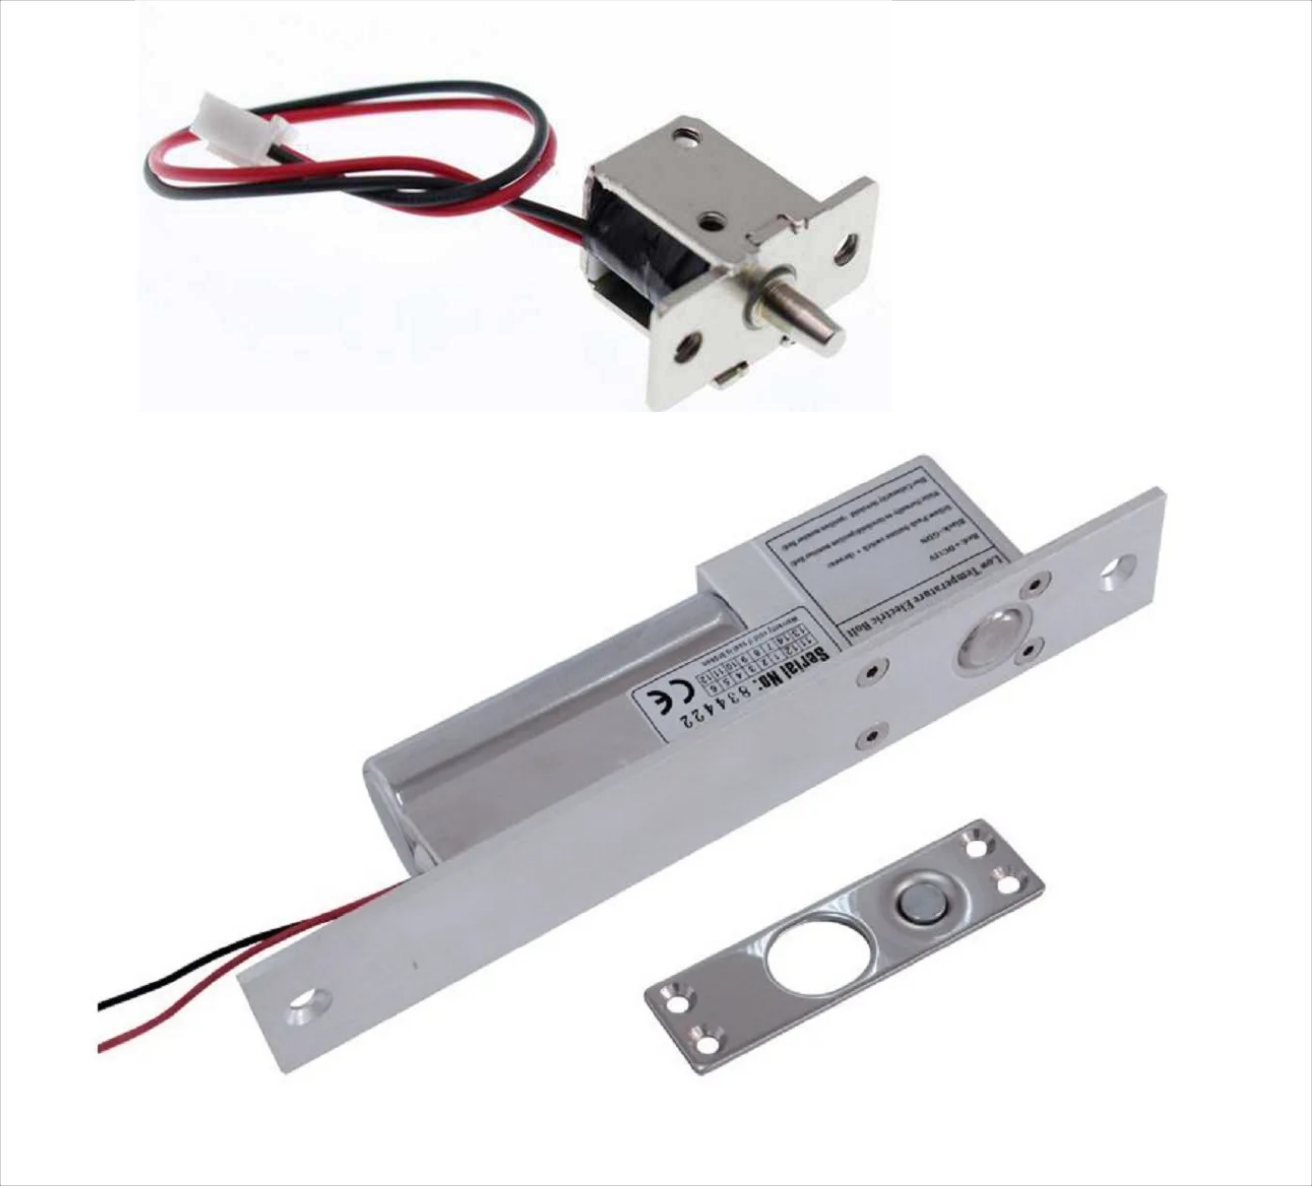
\includegraphics[width=0.5\textwidth]{Pictures/sol+perno.png}
	\rule{35em}{1pt}
	\caption[Cerramientos de perno]{Se muestran ejemplos de cerramientos eléctricos que funcionan con solenoide y perno. }
	\label{fig:sol+perno}
\end{figure}

\subsubsection{Solenoide y Clavija}
De una forma similar a la descripta para el caso del perno, un solenoide se utiliza para formar un pequeño electroimán en el interior del dispositivo. La fuerza inducida deforma de manera elástica una clavija o chapa metálica delgada en forma de ele. Esta deformación libera el mecanismo que bloquea el movimiento del pestillo. Este es el caso del traba-pestillo eléctrico o del pasador eléctrico cuyos ejemplos se muestran en la figura ~\ref{fig:sol+clav}.

\begin{figure}[htbp]
	\centering
	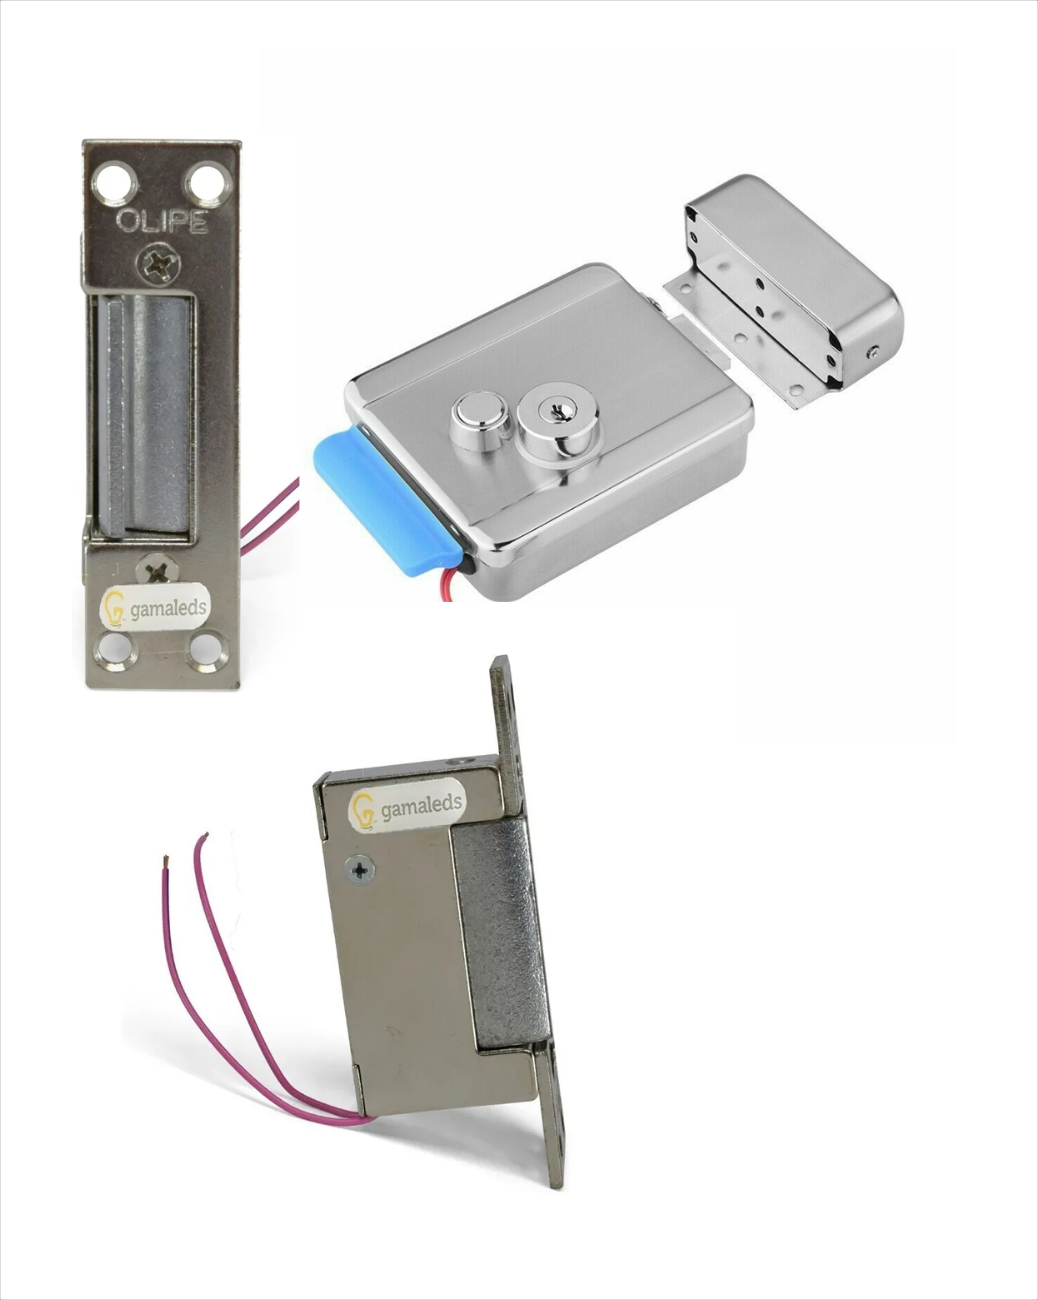
\includegraphics[width=0.35\textwidth]{Pictures/sol+clav.png}
	\rule{35em}{1pt}
	\caption[Cerramientos de perno]{Se muestran ejemplos de cerramientos eléctricos que funcionan con solenoide y clavija. }
	\label{fig:sol+clav}
\end{figure}

\subsubsection{Electroimán}
En esta forma de funcionamiento se construye un electroimán de dimensiones considerables capaz de ejercer una fuerza de atracción magnética cercana a los 300 kgF sobre una chapa metálica que también se incluye como parte del cerramiento. Por lo general incluyen en su circuito una etapa de compensación de factor de potencia para remanencia cero.
Este es el caso de la cerradura por electroimán que se muestra en la figura ~\ref{fig:cerr-mag}.

\begin{figure}[htbp]
	\centering
	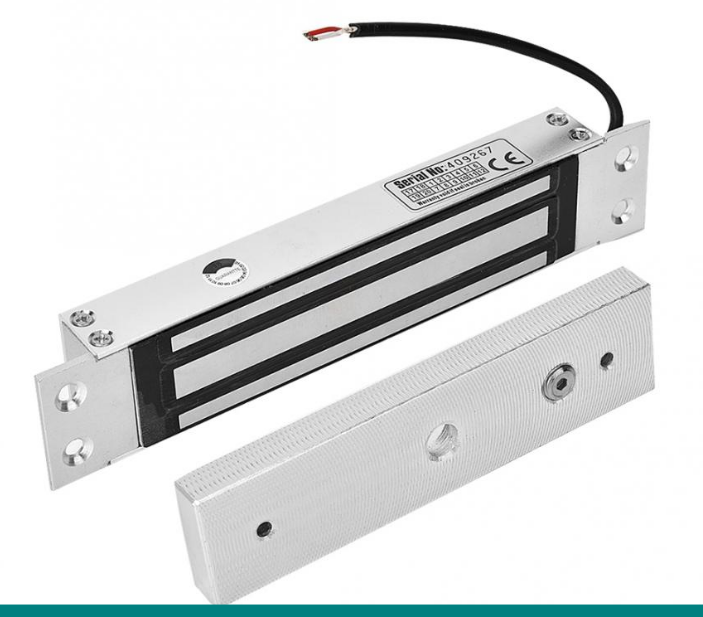
\includegraphics[width=0.4\textwidth]{Pictures/magnet.png}
	\rule{35em}{1pt}
	\caption[Cerradura Electroimán]{Se muestran un ejemplo de cerradura eléctrica que funcionan por electroimán. }
	\label{fig:cerr-mag}
\end{figure}

\subsubsection{Motor Eléctrico}
Para el caso de grandes portones de garage o acceso vehicular se utilizan motores de corriente alterna o brushless de corriente contínua con su respectivos controladores. Estos motores interactúan mecánicamente con otras interfaces mecánicas instaladas en las aperturas para posibilitar la tarea de apertura o cierre. Adicionalmente es necesario la incorporación de sensores que indiquen el estado del sistema y aseguran su correcto funcionamiento.
Todos los tipos de automatización de portones así como los sistemas de apertura con cortinas metálicas comparten el mismo principio de funcionamiento y utilizan motores similares al que se muestra en la figura ~\ref{fig:motorport}.

\begin{figure}[htbp]
	\centering
	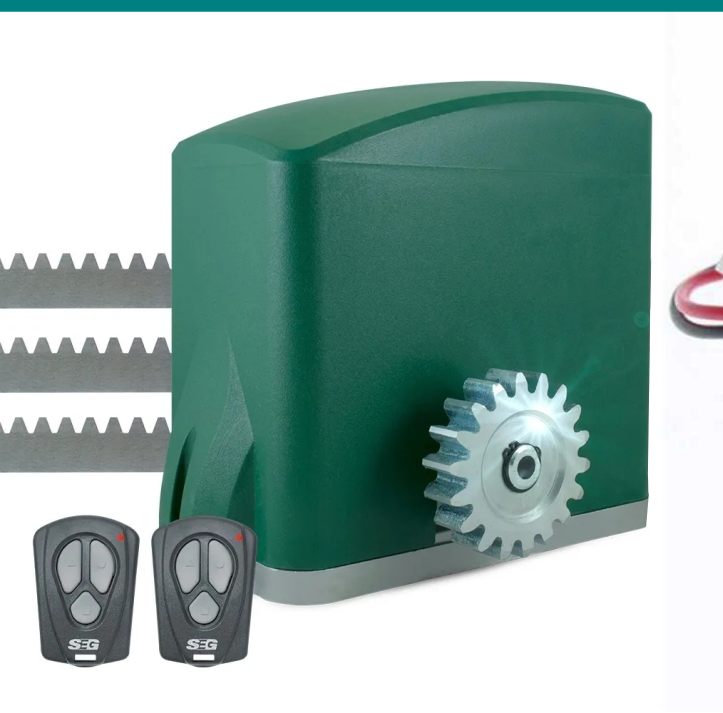
\includegraphics[width=0.4\textwidth]{Pictures/motor.png}
	\rule{35em}{1pt}
	\caption[Motor Portones Automatizados]{Motor empleado en sistemas de automatización de portones de garaje o accesos vehiculares. }
	\label{fig:motorport}
\end{figure}

\section{Controladores}
Todos los cerramientos eléctricos mencionados anteriormente no funcionan por si mismos sino que requieren de un dispositivo controlador.
Algunos ejemplos se muestran en la figura ~\ref{fig:controladoresacceso}.\\
\begin{figure}[htbp]
	\centering
	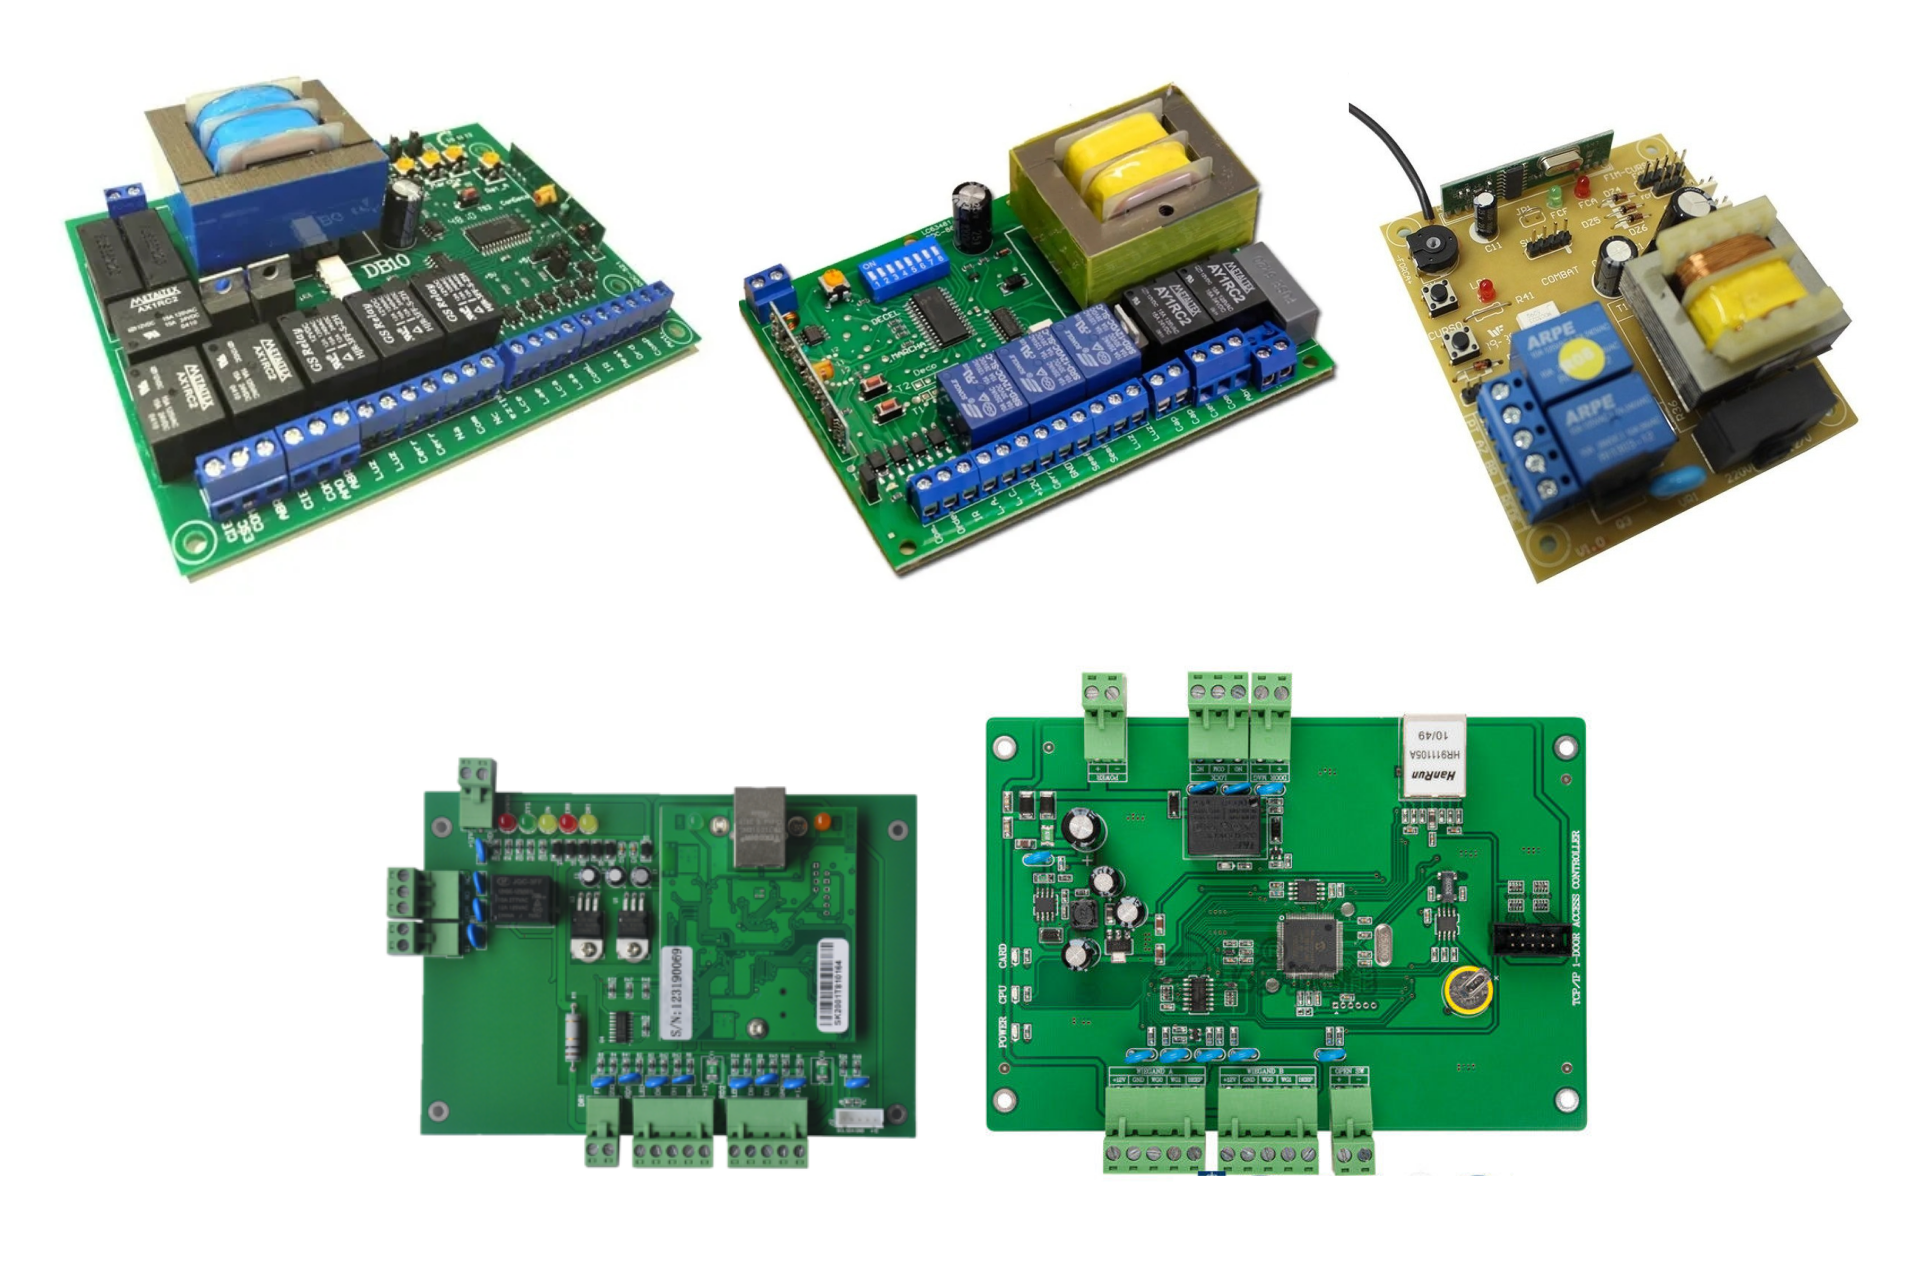
\includegraphics[width=0.8\textwidth]{Pictures/controladoresacceso.png}
	\rule{35em}{1pt}
	\caption[Controladores de Acceso]{Algunos ejemplos de controladores de cerramientos eléctricos.}
	\label{fig:controladoresacceso}
\end{figure}
Estos controladores son circuitos electrónicos que se encargan de generar las señales de activación y/o control de los cerramientos eléctricos. El usuario podrá actuar sobre el cerramiento eléctrico a través de diversos modos de accionamiento, se mencionan los más habituales:
\begin{itemize}
	\item Portero telefónico
	\item Contraseña por teclado
	\item Lector biométrico
	\item Llave electrónica
	\item Botón externo
\end{itemize}

Para dar soporte a una o múltiples formas de accionamiento el controlador ofrece una interfaz de configuración y los componentes necesarios para su operación.
En el caso de los cerramientos a motor es necesario incluir sensores de apertura y funcionamiento.

\subsection{Sensores}
Por lo general solo son empleados por los controladores para cerramientos a motor. Existen vario tipos de sensores para estos controladores se mencionan los más utilizados:
\begin{itemize}
	\item Sensores de Fin de Carrera
	\item Encoder Digital
\end{itemize}
. 
\subsubsection{Sensores de Fin de Carrera}
\label{section:fincarrera}
Se utiliza el plural para este caso de sensado porque se utilizan de a pares. Se trata de un par de sensores binarios que indican apertura o cierre total del cerramiento.
Suelen venir en dos presentaciones con modo de funcionamiento distinto.\\
\textbf{Por proximidad magnética:} En este caso cada uno de los sensores está compuesto por un imán permanente y un switch encapsulado como se muestra en la figura ~\ref{fig:fincarrera}(a). Este encapsulado contiene en su interior un filamento de material ferromagnético flexible que al aproximarse lo suficiente al imán se desplaza y cierra el circuito.\\
\textbf{Por choque mecánico:} Estos sensores son switches mecánicos muy sensibles que se instalan en los límites del marco de la abertura y al mínimo contacto con la parte móvil cierran sus circuitos. En la figura ~\ref{fig:fincarrera}(b) se muestran ejemplos de estos dispositivos.

\begin{figure}[htbp]
	\centering
	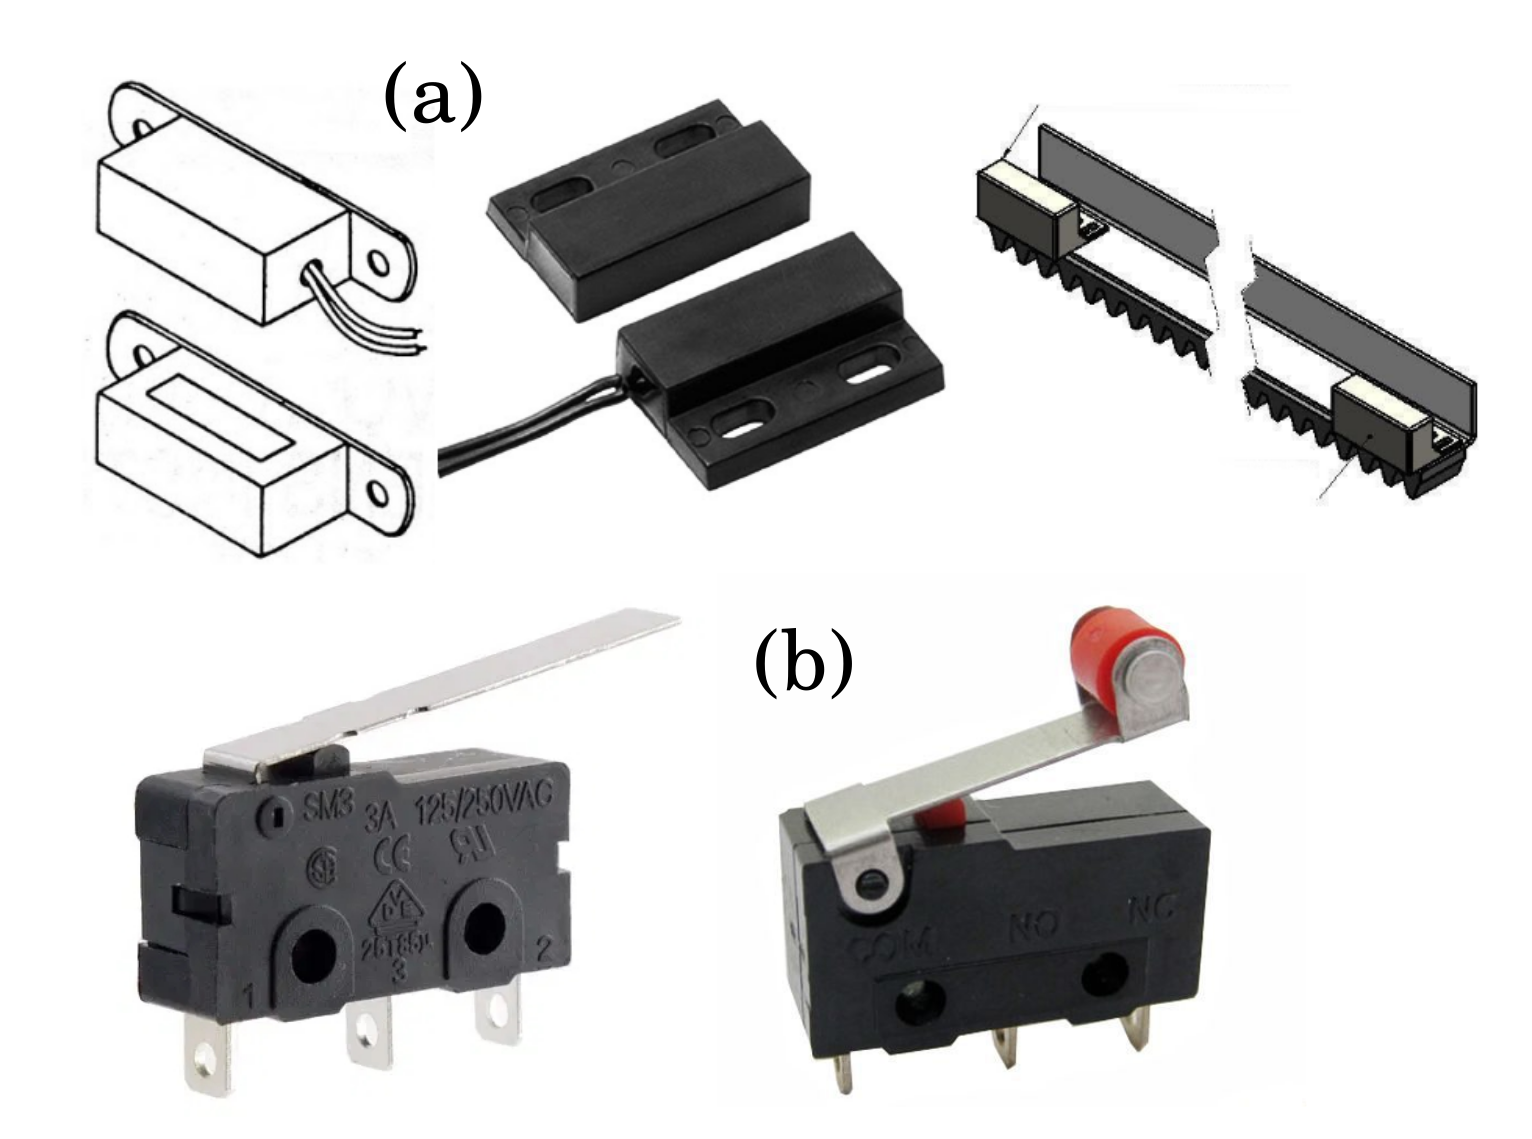
\includegraphics[width=0.6\textwidth]{Pictures/fincarrera.png}
	\rule{35em}{1pt}
	\caption[Sensores de fin de carrera]{Ejemplos de sensores de fin de carrera.(a) Sensores por proximidad magnética, (b) Sensores por choque mecánico. }
	\label{fig:fincarrera}
\end{figure}

\subsubsection{Encoder Rotativo}
Un encoder es un sensor de movimiento mecánico que genera señales digitales en respuesta al movimiento y puede proveer  información sobre la posición, la velocidad y la dirección del movimiento. En particular el econder rotativo responde al movimiento de rotación de un eje. Por lo general los controladores de cerramientos eléctricos a motor utilizan encoders rotativos incrementales que generan un tren de pulsos que se puede utilizar para determinar la posición y la velocidad del eje del motor. En la figura ~\ref{fig:encoder00} se observa la forma del tren de pulsos que genera el encoder.

\begin{figure}[htbp]
	\centering
	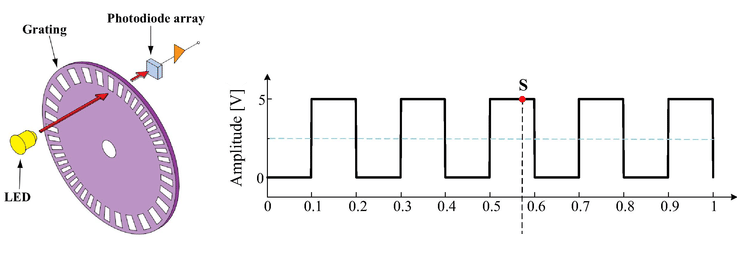
\includegraphics[width=0.8\textwidth]{Pictures/encoder00.png}
	\rule{35em}{1pt}
	\caption[Encoder Rotativo]{Ilustración simplificada de un encoder rotativo con salida de onda cuadrada TTL. }
	\label{fig:encoder00}
\end{figure}


\subsection{Monitoreo y Alerta}
La mayoría de los controladores poseen interfaces que permiten la conexión local de luminarias testigo, así como bocinas de alerta. Algunos modelos incluyen un puerto serie (RJ45, RJ14) capaz de comunicarse mediante comandos estándar con los tradicionales sistemas de alarma.

\subsubsection{Monitoreo Remoto}
Al momento de iniciar el presente proyecto integrador no existían controladoras de acceso con la funcionalidad de monitoreo remoto incorporada de fábrica.
La alternativa para tener información del cerramiento eléctrico y el estado de la abertura que opera consiste en instalar un sensor de apertura y conectarlo a una central de alarma. Estos sensores son baratos y su principio de funcionamiento coincide con el descripto para los sensores de fin de carrera y que se puede consultar en la sección ~\ref{section:fincarrera}.
Las centrales de alarma suelen estar conectadas por cableado telefónico a un servicio de monitoreo que lanza las notificaciones pertinentes según se hayan configurado.
Una basta mayoría de proveedoras de servicio de monitoreo de alarmas ahora ofrecen plataformas web o aplicaciones móviles que permiten el monitoreo de las centrales en tiempo real.

\subsection{Llaves Electrónicas y Control Remoto}
Actualmente la mayoría de los controladores de acceso soportan algún tipo de llave electrónica.
Una llave electrónica es un dispositivo electrónico que le permite al usuario operar el cerramiento eléctrico. Existen diversos tipos de llaves electrónicas a continuación se mencionan las más utilizadas.
\begin{itemize}
	\item Llaves RFID
	\item Control Remoto RF
\end{itemize}

\subsubsection{Llaves RFID}
RFID (Radio-frequency identification) es un sistema de almacenamiento y recuperación de datos a distancias cortas por emisión de radiofrecuencia de baja potencia. 
Una etiqueta RFID consiste en un pequeño circuito receptor y transmisor de radio. Cuando es activada por un pulso de interrogación electromagnético emitido por un dispositivo lector RFID cercano, la etiqueta transmite datos digitales de vuelta al lector, generalmente un número identificador.
Estas etiquetas o circuitos RFID son tan diminutos que pueden incluirse en objetos de tamaño reducido como llaveros y tarjetas, algunos ejemplos se muestran en la figura ~\ref{fig:llavesrfid}.
El usuario del sistema de acceso aproximará esta llave al lector RFID incluido en el controlador y se producirá el intercambio del número identificatorio. En caso de que ese dato esté registrado en el controlador el usuario podrá controlar el cerramiento eléctrico.

\begin{figure}[htbp]
	\centering
	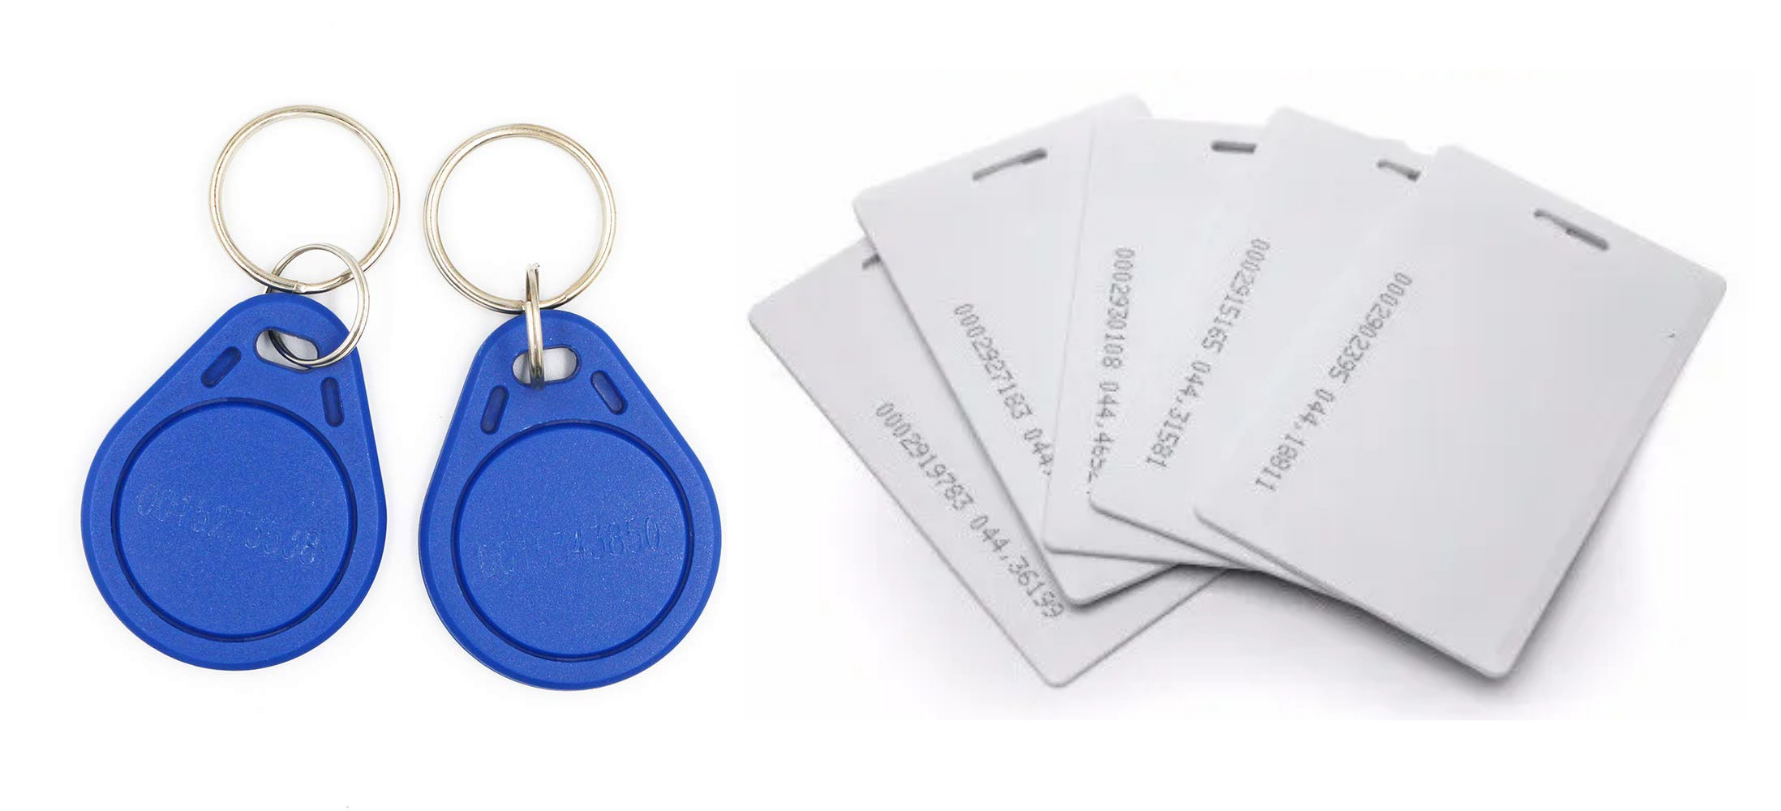
\includegraphics[width=0.8\textwidth]{Pictures/llavesrfid.png}
	\rule{35em}{1pt}
	\caption[Llaves RFID]{Llaveros y tarjetas con etiquetas RFID. }
	\label{fig:llavesrfid}
\end{figure}

\subsubsection{Control Remoto RF}
RF es el acrónimo de Radio-Frequency y hace referencia a las tecnologías que emplean sistemas de comunicación por emisión de ondas electromagnéticas. Por lo general se utilizan anchos de bandas libres sin restricciones gubernamentales con baja potencia de transmisión.
En el caso del control remoto para por RF un código numérico identificatorio se transmite al controlador que incluye un circuito receptor comúnmente en las frecuencias que van de los 200 MHz a los 500 Mhz. El rango de acción de estos dispositivos es de aproximadamente 100 mts en línea de visión.
El controlador de acceso permite la actualización del código identificatorio en caso de que ya esté empleado al momento de la configuración. En algunas implementaciones este código es rotatorio y cambia con el uso.
En la figura ~\ref{fig:controlesrf} se muestran algunos ejemplos.

\begin{figure}[htbp]
	\centering
	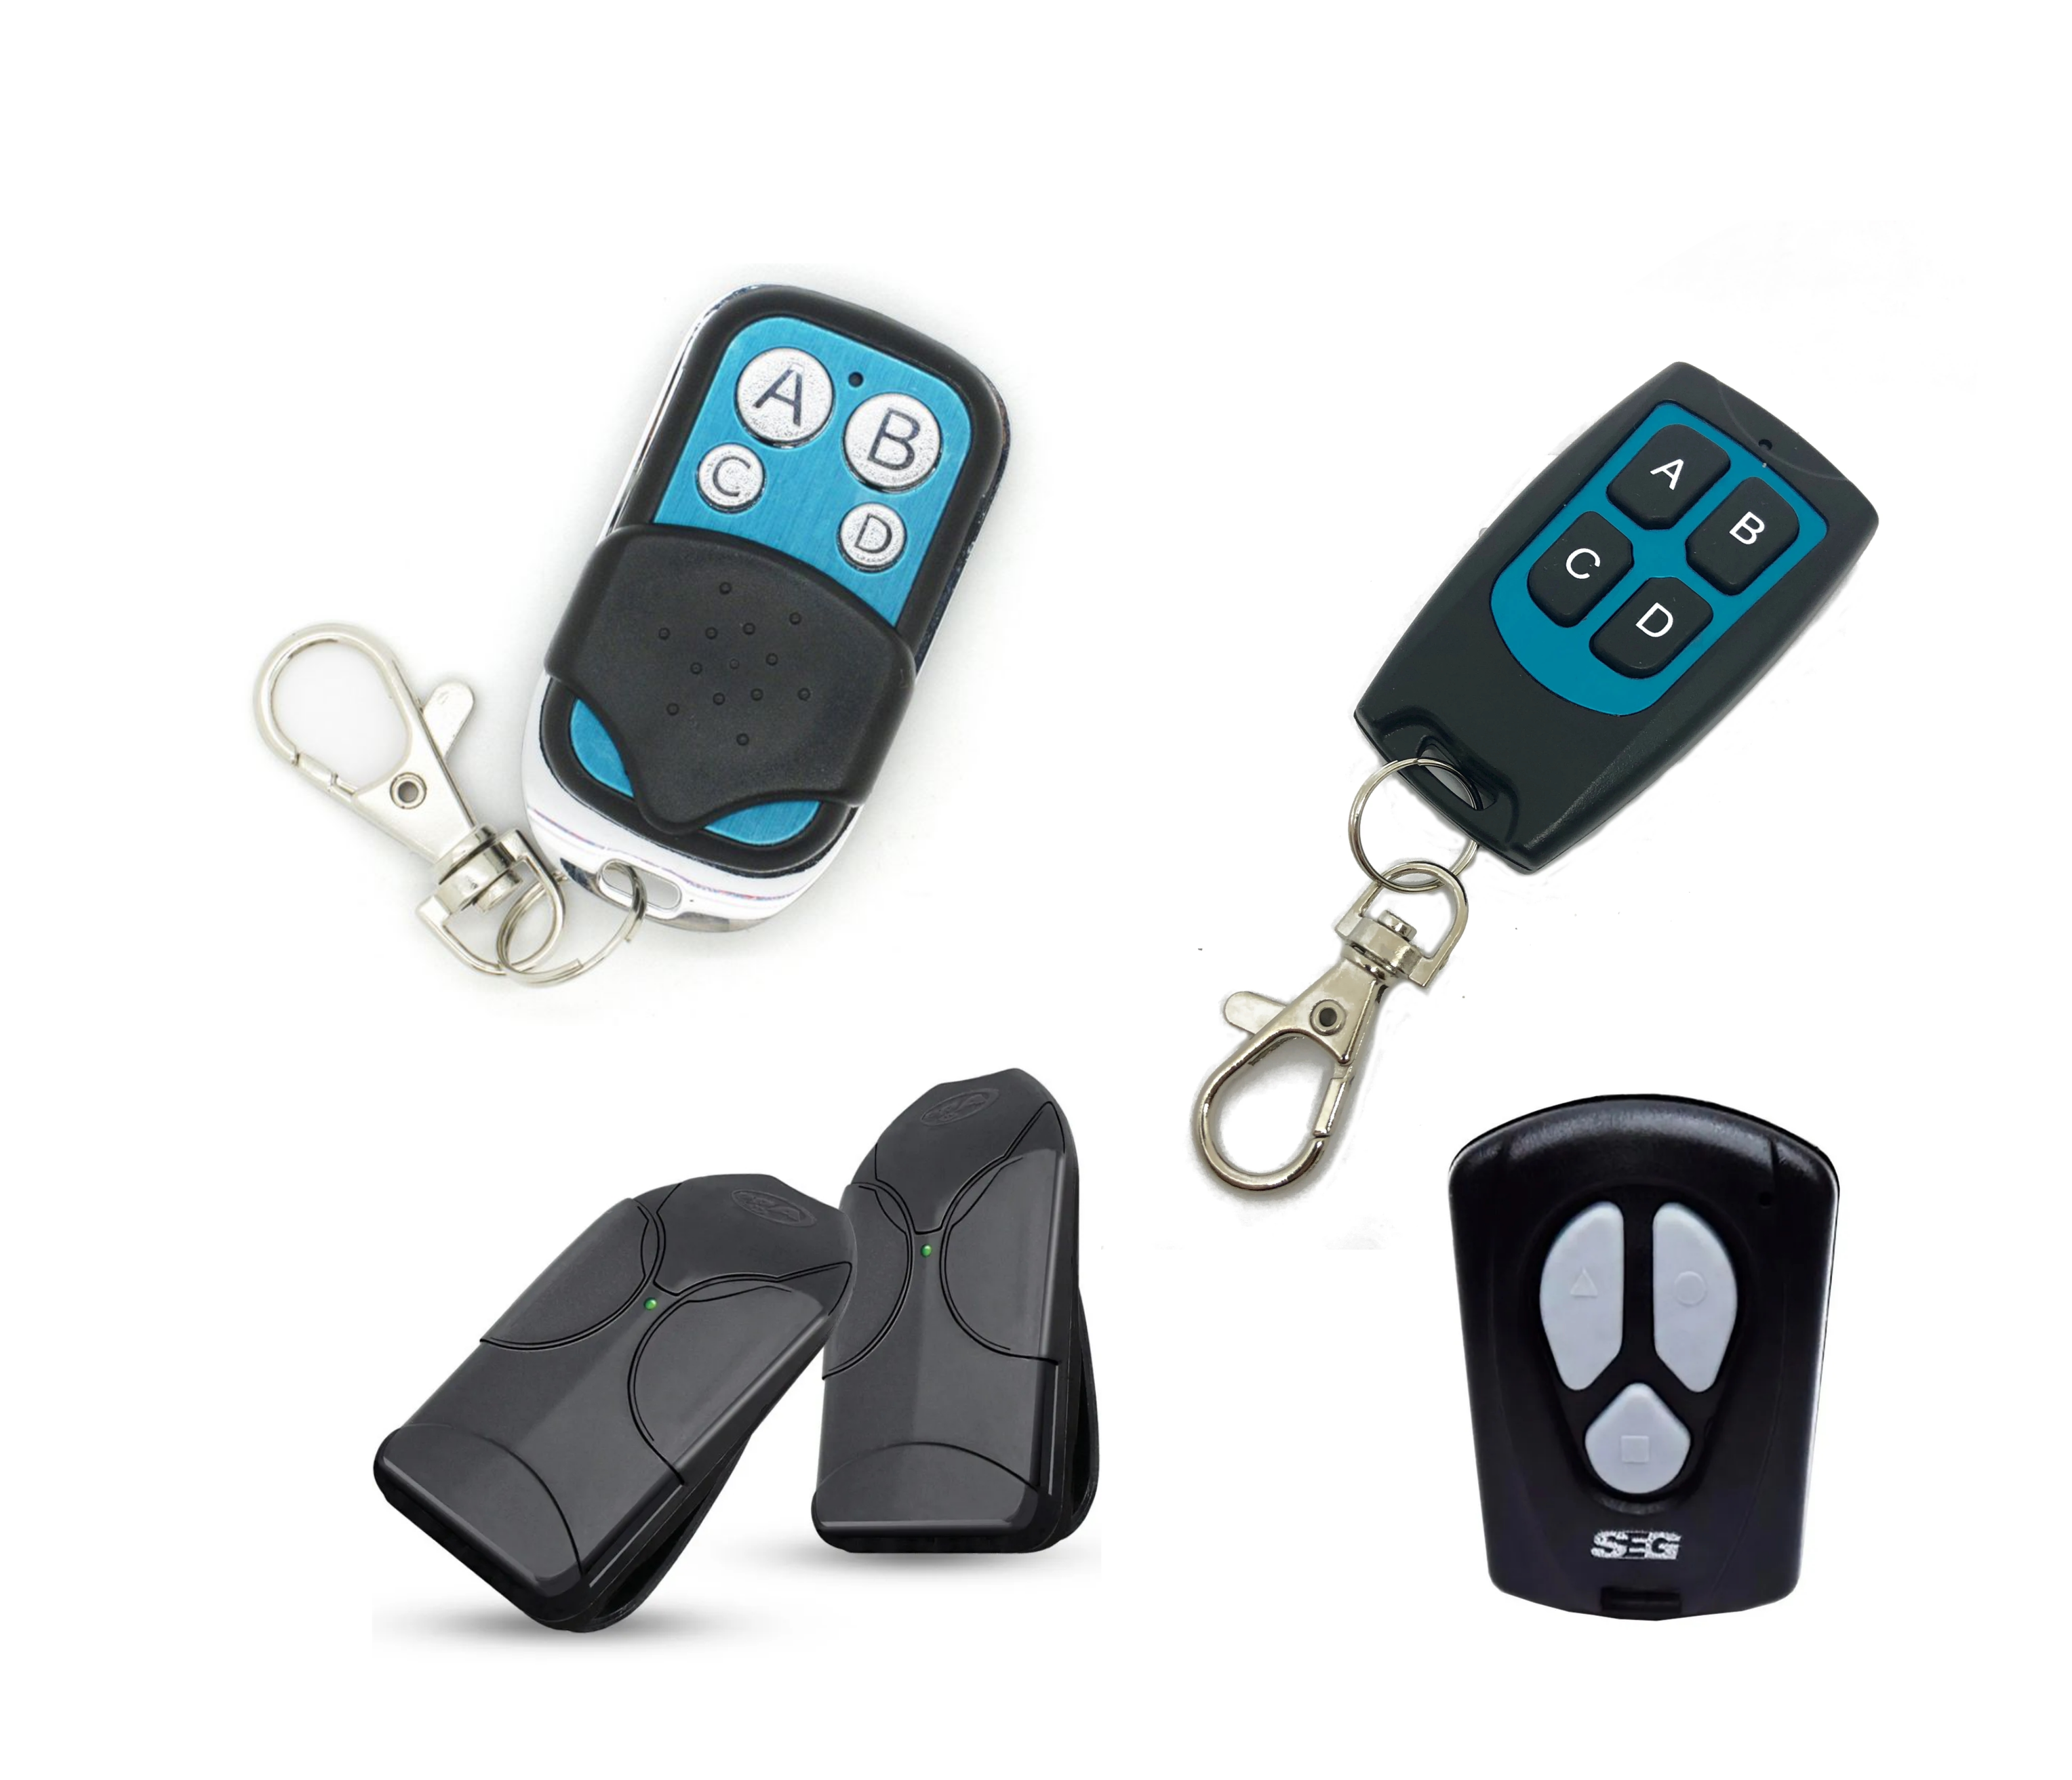
\includegraphics[width=0.6\textwidth]{Pictures/controlesrf.png}
	\rule{35em}{1pt}
	\caption[Controles RF]{Controles remotos RF en diferentes presentaciones. }
	\label{fig:controlesrf}
\end{figure}

\subsubsection{Un problema de seguridad}
Tanto el empleo de llaves RFID como controles RF presentan un problema de seguridad para estos sistemas de acceso electrónico ya que conceden acceso a quien porta llave sin importar si se trata del dueño real.
En ningún caso se utilizan protocolos para la identificación del solicitante. Así mismo tampoco se emplean algoritmos de  encripción de datos por lo que el código de identificación se transmite en texto plano, por lo menos este es el caso para la mayoría de las implementaciones.\\
Por esta razón existen métodos de hacking ya documentados que involucran dos técnicas principales.\\
\textbf{Clonado por lectura RFID:} En este caso simplemente basta con tener un lector RF y acceso a la etiqueta RFID empleada por la llave a ser clonada. Una vez leído el código se crea una etiqueta con el mismo código y se obtiene acceso.\\
\textbf{Clonado por intercepción RF:}  Ésta técnica implica un ataque por sniffing del código de identificación. Teniendo en cuenta que la frecuencia y el tipo de modulación empleado por los sistemas actuales son conocidos, resulta en una tarea sencilla empleando un transeptor RF y un decodificador por software.\\
\textbf{Inhibición de Señal:} Esta técnica es quizás la mas sencilla de todas. Se utiliza para vulnerar los sistemas de acceso que emplean controles remotos RF. Implica la utilización de un transmisor que contamina con ruido el ancho de banda de operación del control remoto. De esta forma se impide la correcta comunicación con el controlador del cerramiento al momento de enviar la señal de cierre, evitando así que la abertura pueda ser cerrada.

\section{Cerramientos Electrónicos IoT}
IoT (Internet of Things) describe la red de objetos físicos que incorporan circuitos con microcontroladores, software embebido, sensores y componentes de comunicación con el propósito de intercambiar datos con otros objetos conectados y servicios en linea a través de internet.
Teniendo en cuenta que las aberturas de un edificio son objetos físicos y que los cerramientos eléctricos ofrecen un modo de accionamiento electrónico para estos objetos, es posible concebir la adaptación de los mismos para convertirlos en implementaciones IoT.
Con el ánimo de ilustrar el panorama de productos IoT orientados a la seguridad y al control de acceso se mencionan las categorías más relevantes.

\begin{itemize}
	\item Smart Alarms
	\item Smart Door Locks
	\item Smart Garage Doors
\end{itemize}

\subsection{Smart Alarms}
Estos productos proponen la instalación y configuración de una red de sensores (comúnmente inalámbricos) en el interior y alrededor del hogar o cualquier edificio en general. Algunos ejemplos de estos sensores se listan a continuación:
\begin{itemize}
	\item Sensores de Humo
	\item Sensores de gases peligrosos (CO2, CO, propano, butano, metano).
	\item Sensores de presencia IR.
	\item Sensores de apertura para puertas y ventanas.
\end{itemize} 
Estos sensores son sistemas embebidos de tamaño reducido con poca capacidad de cómputo y de muy bajo consumo eléctrico incluso en algunas versiones alimentados a baterías.
Por esta razón se emplean protocolos de comunicación acorde a las capacidades de estos dispositivos tales como \textit{zigbee} y \textit{Thread} ambos basados en la especificación IEEE 802.15.4 por lo que sus respectivos stacks de software presentan footprints de memoria adecuados para la aplicación en particular.\\
Como parte fundamental de la red se incluye un dispositivo electrónico denominado \textit{concentrador, gateway ó central} que posee al menos dos interfaces de comunicación principales, una para conectarse a la red de sensores y otra para acceder a internet. Este ''gateway'' recibe las actualizaciones de estado de los sensores y las reenvía por internet a un servicio de monitoreo mantenido por el mismo proveedor.\\
El usuario puede acceder a los datos almacenados por el servicio a través de un cliente web o aplicación móvil.
Adicionalmente estos clientes ofrecen una GUI para la configuración tanto de la central como para los sensores.
En la figura ~\ref{fig:smartalarms} se muestran ejemplos de los productos ofrecidos por los fabricantes más populares.

\begin{figure}[htbp]
	\centering
	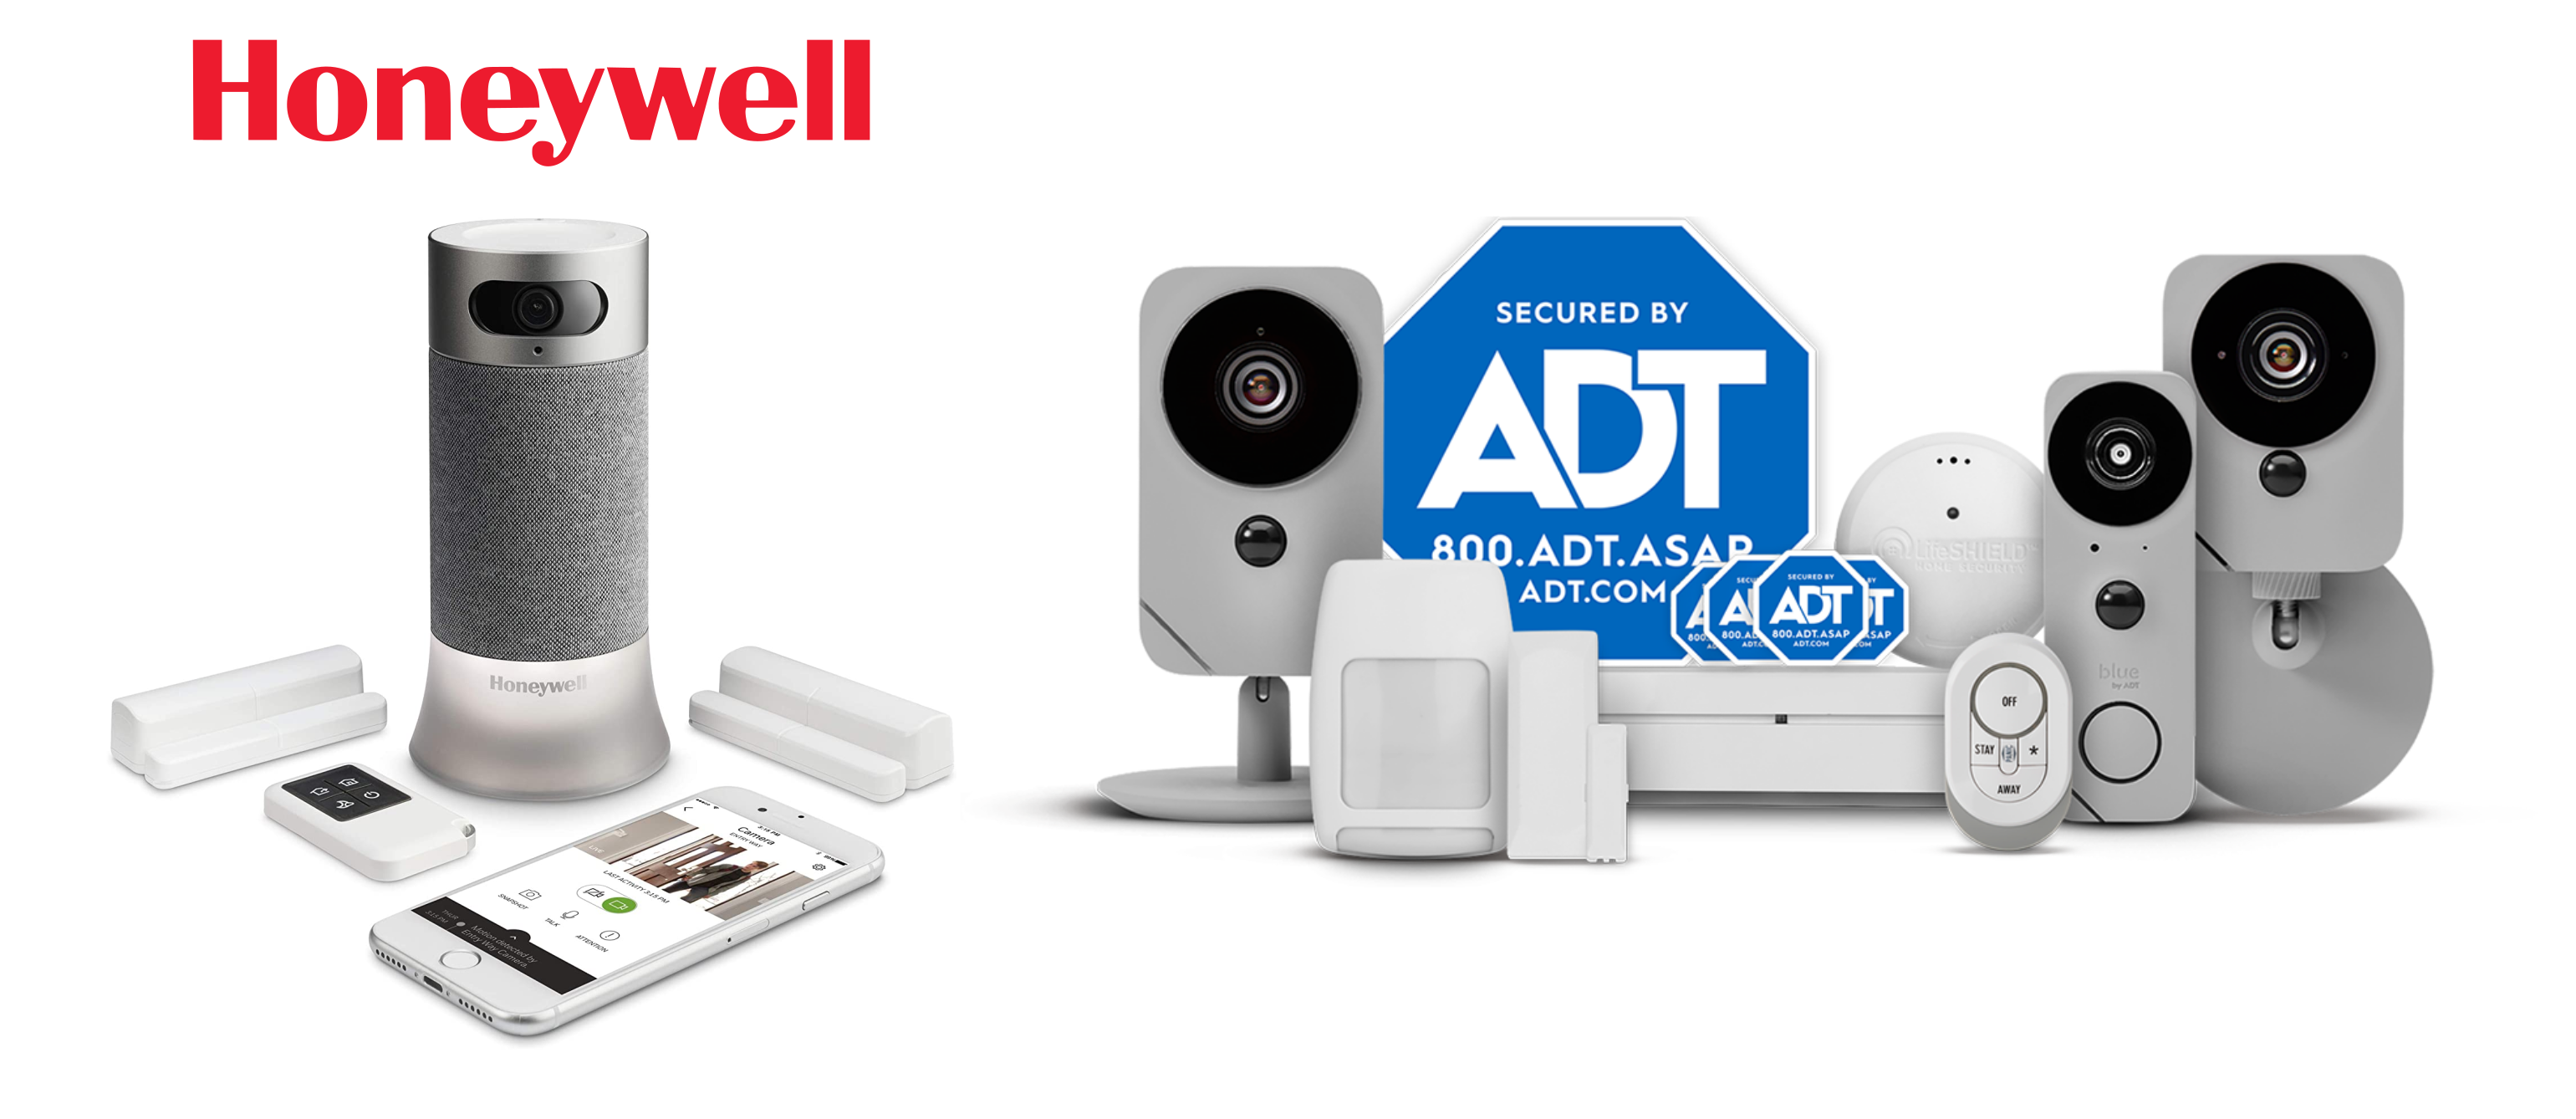
\includegraphics[width=0.8\textwidth]{Pictures/smartalarms.png}
	\rule{35em}{1pt}
	\caption[Smart Alarms]{Familia de productos de los fabricantes mas conocidos.}
	\label{fig:smartalarms}
\end{figure}

\subsection{Smart Door Locks}
Esta categoría de productos comprenden dispositivos electromecánicos que reemplazan o se adaptan a las tradicionales cerraduras de tambor radial comúnmente utilizadas en puertas residenciales estadounidenses.
Estos dispositivos incluyen el sistema embebido capaz de conectarse a internet a través de WiFi o Bluetooth (mediante el uso de un gateway WiFi como en el caso de SESAME).
Para todos los casos se ofrece una aplicación móvil que hace de llave virtual y permite el acceso a estos cerramientos inteligentes.
Adicionalmente el usuario administrador podrá agregar y remover usuarios autorizados a operar el dispositivo.
En la figura ~\ref{fig:smartlocks} se pueden observar ejemplos reales de productos disponibles en el mercado.

\begin{figure}[htbp]
	\centering
	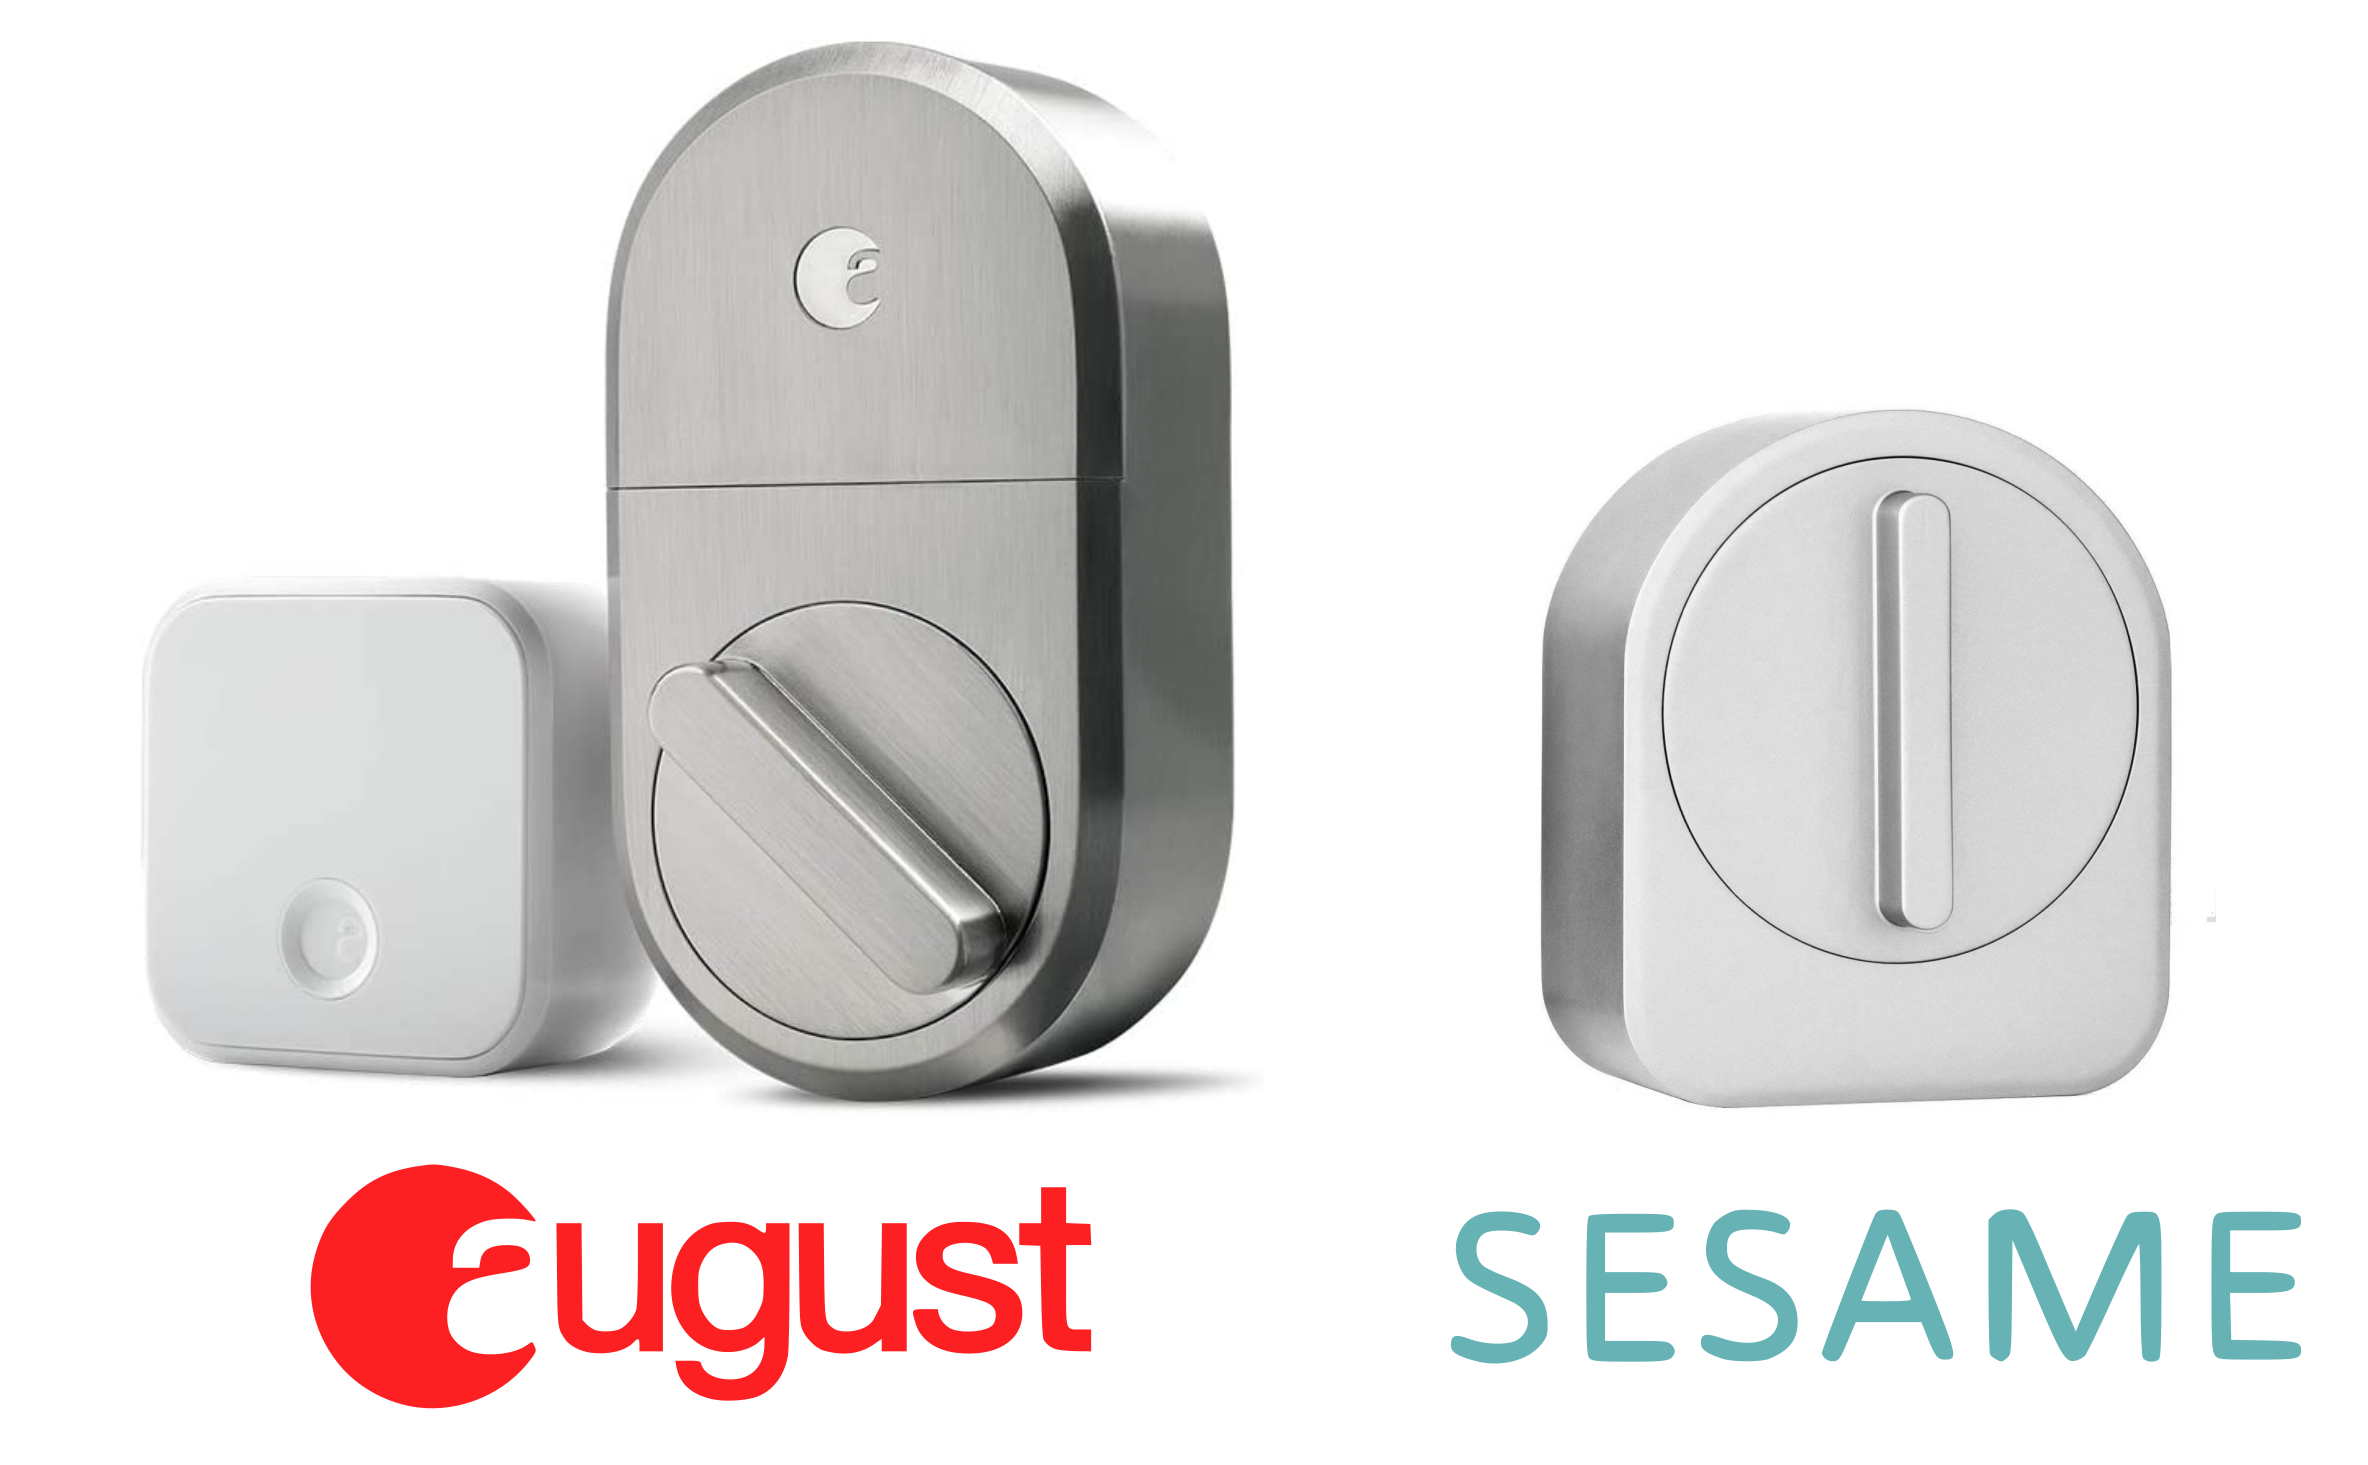
\includegraphics[width=0.6\textwidth]{Pictures/smartlocks.png}
	\rule{35em}{1pt}
	\caption[Smart Locks]{Modelos más comercializados de cerraduras inteligentes.}
	\label{fig:smartlocks}
\end{figure}

\subsection{Smart Garage Door}
Para el caso de los portones automatizados de garaje existen diversas implementaciones que agregan estos objetos a la familia de productos IoT.\\
La mayoría de los controladores ofrecen al menos una interfaz para conexión de un botón externo de apertura y cierre. Por esta razón diversas sturtups desarrollaron implementaciones de dispositivos a modo de accesorios compatibles con una familia de controladores. Este es el caso de ISmartGate, Nexx NXG-100 y Garadget.\\
Luego los fabricantes más importantes de controladores y motores para portones de garaje de estados unidos realizaron sus propias implementaciones y las incorporaron a sus controladores como una funcionalidad built-in. Este es el caso de la empresa Genie con su linea de productos Aladdin. Por otro lado la empresa Chamberlane optó por el enfoque de agregar la misma funcionalidad mediante el uso de accesorios que ofrecen con su línea myQ.\\
Mas recientemente, en el transcurso del año 2019 PPA, la empresa más grande de Sudamérica especializada en automatización de aberturas residenciales e industriales. Presentó un gateway IoT (SPIRIT) compatible con una amplia familia de sensores y actuadores que también fabrican. Entre ellos un módulo que permite el accionamiento y monitoreo remoto de portones automatizados.
Todas las implementaciones ofrecen una aplicación móvil que se usará para el monitoreo, control y configuración del producto.
En la figura ~\ref{fig:smartgates} se muestran ejemplos de estos productos.

\begin{figure}[htbp]
	\centering
	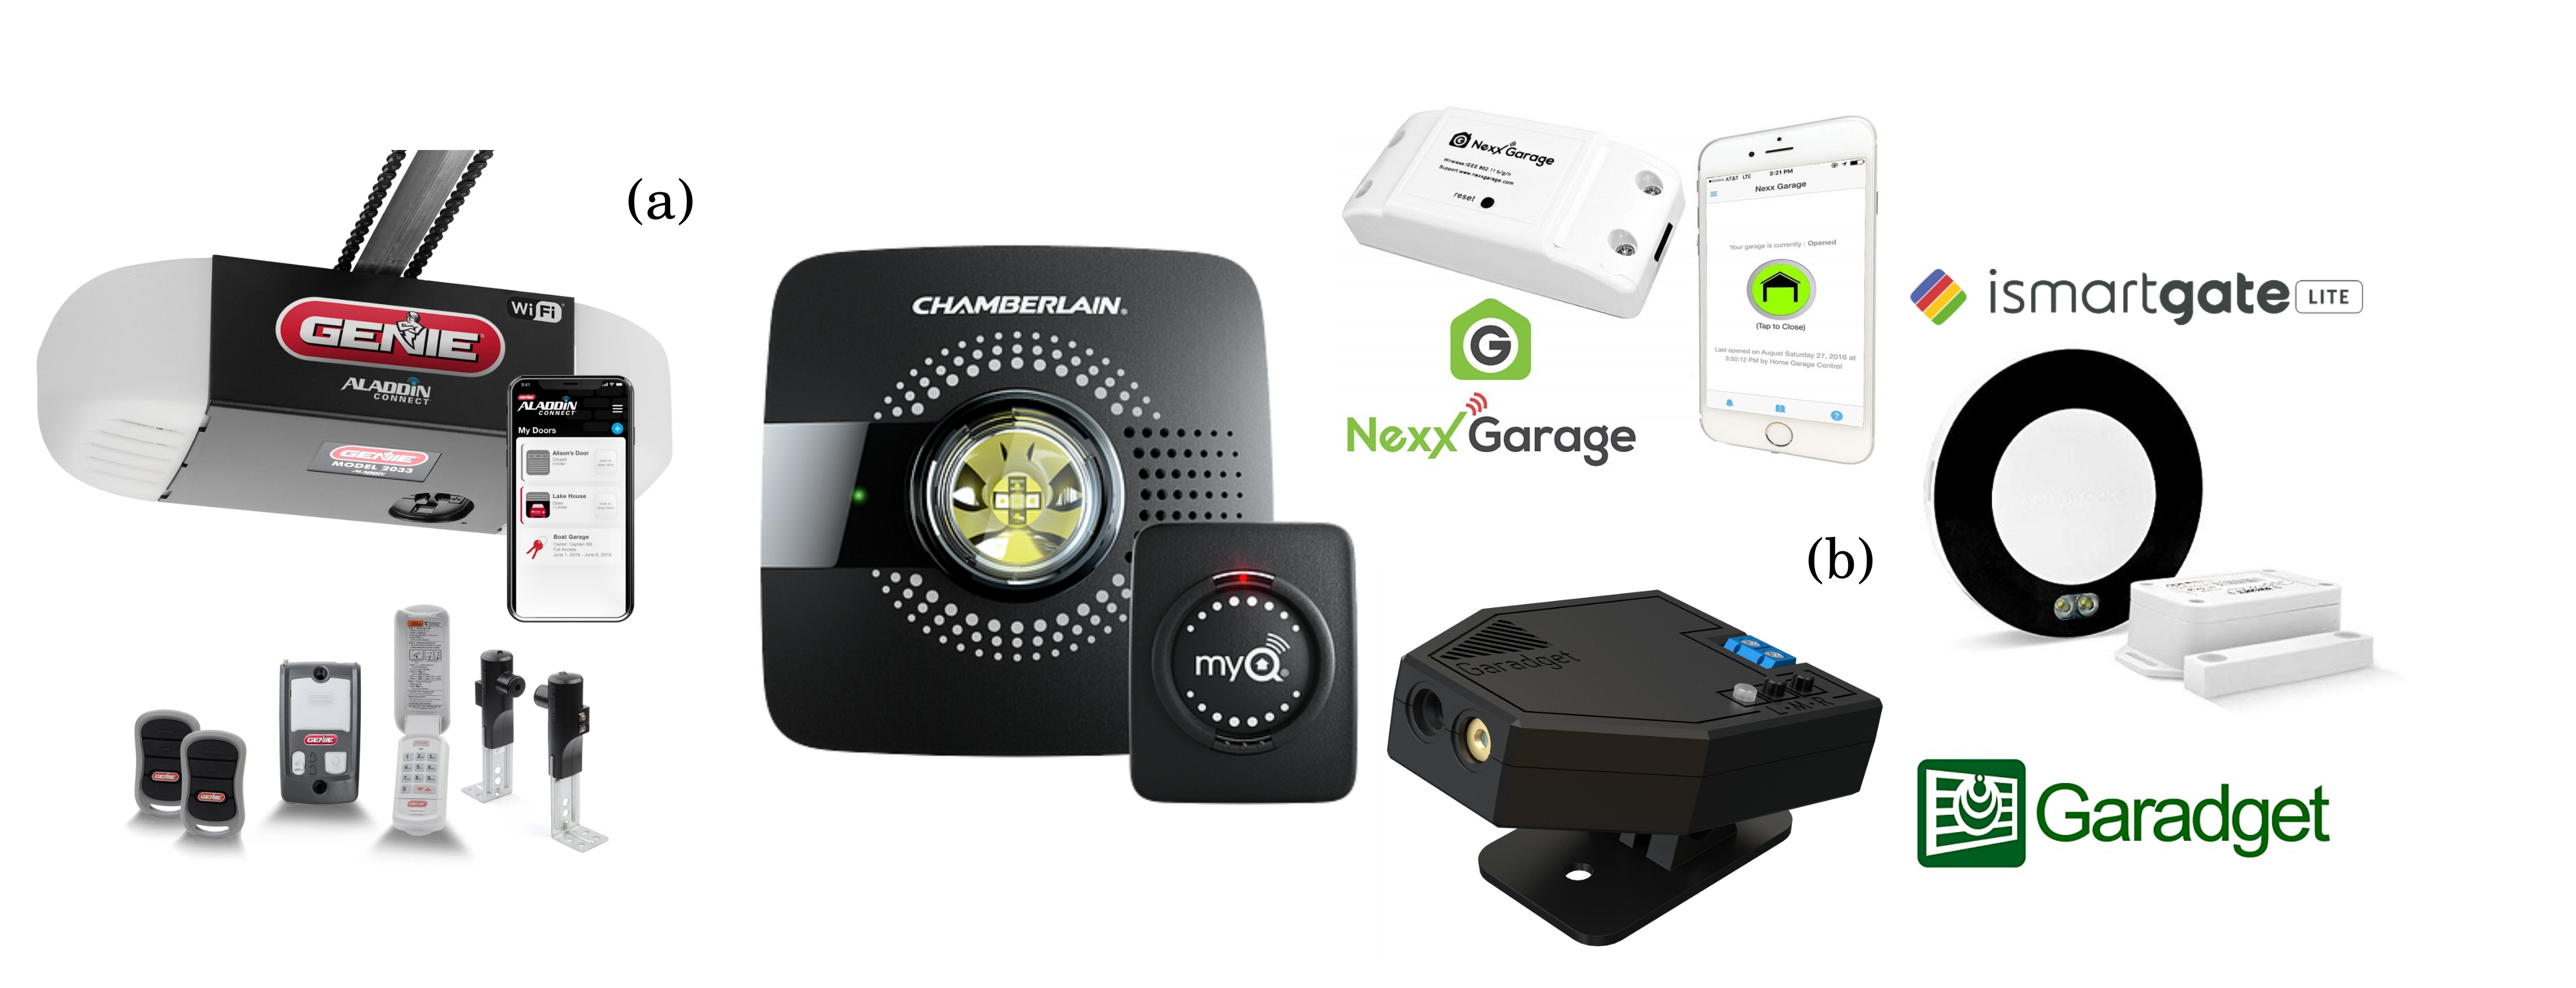
\includegraphics[width=0.8\textwidth]{Pictures/smartgates.png}
	\rule{35em}{1pt}
	\caption[Smart Garage Gates]{Modelos más comercializados de automatización inteligente para portones de garaje.}
	\label{fig:smartgates}
\end{figure}

\section{Conclusión}
Los cerramientos eléctricos presentan una interesante gama de dispositivos para los que pueden plantearse la extensión de funcionalidad con el objetivo de convertirlos en productos IoT. Algunas de las funcionalidades que se entienden deseables para este tipo de dispositivos son el monitoreo remoto, el control a distancia y la configuración remota.\\
Adicionalmente aparece una oportunidad de mejora al plantear los problemas de seguridad que tienen las implementaciones actuales y que podrían ser mitigados al utilizar protocolos de comunicación modernos.
 
%% Chapter Template

\chapter{Desarrollo} % Main chapter title

En el presente capítulo se describe el proceso de desarrollo del sistema que se compone en 3 partes, las cuales se detallan en cada caso el procedimiento de diseño e implementación utilizando como referencia el Documento de Especificación de Requerimientos de Sistema de \textit{Software} propuesto por la \textit{IEEE}.\\

\label{Chapter3} % Change X to a consecutive number; for referencing this chapter elsewhere, use \ref{ChapterX}

\lhead{Capítulo 3. \emph{Desarrollo}} % Change X to a consecutive number; this is for the header on each page - perhaps a shortened title

%----------------------------------------------------------------------------------------
%	SECTION 1
%----------------------------------------------------------------------------------------
\section{Análisis del problema}
El problema consiste en comunicar a través de Internet, notificaciones de alertas producidas por un dispositivo que contiene sensores, hacia un servidor remoto el cual recibe y almacena dichas notificaciones y, eventualmente puede tomar decisiones acerca de las mismas a través de un operador que monitoriza el sistema. \\
Por otro lado, el control del dispositivo se debe realizar a través de un teléfono móvil inteligente(\textit{smartphone}) a través de la red LAN del hogar. Éste, a su vez, puede ser conectado con otros aparatos eléctricos para comandarlos en caso de ser necesario.\\
Por lo tanto, se decidió dividir el problema en 3 partes, las cuales fueron diseñadas para poder ser desarrolladas concurrentemente. Éstas son: Un subsistema encargado de la monitorización de los sensores(alarma), otro que recibe las notificaciones y emite alertas(Servidor) y por último, el encargado de comunicar al usuario con la alarma (aplicación).
\newpage

%% Chapter Template

\chapter{Descripción del modelo experimental} % Main chapter title

\label{Chapter4} % Change X to a consecutive number; for referencing this chapter elsewhere, use \ref{ChapterX}

\lhead{Capítulo  4. \emph{Descripción del modelo experimental}} % Change X to a consecutive number; this is for the header on each page - perhaps a shortened title

Se definieron 3 modelos experimentales, donde los niveles de abstracción fueron disminuyendo hasta el último, donde se realizaron las pruebas en condiciones reales.\\
El primer modelo, el virtual, representa el sistema en su totalidad en un entorno local, simulando los subsistemas a través de módulos de software.\\
El siguiente fué el modelo físico, donde en cada subsistema se utilizó sobre la arquitectura de \textit{hardware} correspondiente, pero en un entorno de red local.\\
Una vez comprobado que el sistema actuó correctamente en un ambiente físico real aunque limitado, se continuó con el último modelo que fué el real. En este caso, cada sistema se ejecutó en su ambiente real sin limitaciones de conectividad y con la totalidad de sus funcionalidades.\\
En las siguientes secciones se detallan las características de cada modelo.


\newpage


%----------------------------------------------------------------------------------------
%	SECTION 1
%----------------------------------------------------------------------------------------

\section{Modelo virtual}

Como se muestra en la figura \ref{Diagrama_virtual}, este modelo consiste  en probar los subsistemas a través de módulos de \textit{software} ejecutados en la misma computadora, que simulaban el sistema real:\\

\begin{figure}[htbp]
	\centering
		\includegraphics[width=0.8\textwidth]{Figures/Diagrama_virtual.png}
		\rule{35em}{1.5pt}
	\caption[Modelo Virtual del sistema]{Modelo Virtual del sistema}
\label{Diagrama_virtual}
\end{figure}

\begin{figure}[htbp]
	\centering
		\includegraphics[width=1\textwidth]{Figures/captura_virtual.png}
		\rule{35em}{1.5pt}
	\caption[Captura de pantalla de modelo virtual del sistema]{Captura de pantalla de modelo virtual del sistema}

\end{figure}

A continuación se detalla las funcionalidades básicas propias y de comunicación con el resto de los subsistemas, indicando también, sus limitaciones en cada caso.

\newpage


%-----------------------------------
%	SUBSECTION 1.1
%-----------------------------------
	\subsection{Módulo Alarma}

En el caso de la alarma, se desarrolló un programa en C, que simula las alertas y envía notificaciones al servidor.\\
Limitaciones:
\begin{itemize}
\item Recibe órdenes (activar/desactivar) que simplemente limitan al envío de las notificaciones.
\item No se provee autenticación ni cuenta con salidas para comandar.
\end{itemize}


%-----------------------------------
%	SUBSECTION 1.2
%-----------------------------------

	\subsection{Módulo Servidor}

El servidor, realizado en Ruby sobre el \textit{framework Rails}, integra un \textit{script} que recibe notificaciones por \textit{socket} desde la alarma y las muestra en un servidor \textit{web}.\\
Limitaciones:
\begin{itemize}
\item La interfaz gráfica se limita la exposición de las notificaciones en texto plano.
\item El modelo de la base de datos contempla una única tabla donde se resguardan todos los datos.
\item El controlador del servidor WEB no permite realizar CRUD sobre los datos de los usuarios.
\end{itemize}

%-----------------------------------
%	SUBSECTION 1.3
%-----------------------------------

	\subsection{Módulo Aplicación}

Consta de un \textit{software} hecho en Java sobre el \textit{IDE Android Studio}, que envía ordenes por socket a la alarma y recibe las respuestas de la misma.\\
Limitaciones:
\begin{itemize}
\item Este programa se ejecuta sobre un emulador de teléfonos Android.
\item No permite autenticación.
\end{itemize}

\newpage

%----------------------------------------------------------------------------------------
%	SECTION 2
%----------------------------------------------------------------------------------------

\section{Modelo físico}

Una vez comprobada la funcionalidad en el ambiente virtual, se pasó a un ambiente físico controlado y limitado.
El mismo se representa en la figura \ref{Diagrama_fisico}:

\begin{figure}[htbp]
	\centering
		\includegraphics[width=0.8\textwidth]{Figures/Diagrama_fisico.png}
		\rule{35em}{1.5pt}
	\caption[Modelo Físico del sistema]{Modelo Físico del sistema}
\label{Diagrama_fisico}
\end{figure}

Se puede ver que la ejecución del sistema, si bien es sobre la arquitectura correspondiente, la conectividad es limitada a un ambiente de red local y las funcionalidades de cada subsistema no contemplan aún la totalidad de los requerimientos, aunque si los básicos y algunos secundarios.
\newpage


%-----------------------------------
%	SUBSECTION 2.1
%-----------------------------------
	\subsection{Módulo Alarma}

Se desarrolló sobre el microcontrolador K64F, utilizando el \textit{IDE KDS} y el SO \textit{MQX}. \\
Limitaciones:
\begin{itemize}
\item En el caso de los sensores, solo se limitan a interruptores que accionan las alertas, que luego se transmiten en la red local hasta el servidor. 
\item Las notificaciones se restringen a la red local.
\end{itemize}

%-----------------------------------
%	SUBSECTION 2.2
%-----------------------------------

	\subsection{Módulo Servidor}

El servidor se mantuvo en una computadora local, se agregaron funcionalidades \textit{CMS} al servidor \textit{web} para administrar las alarmas y autenticación en las notificaciones entrantes. \\

Limitaciones:
\begin{itemize}
\item Las actualizaciones en la vista del servidor no se realizan automáticamente.
\item Acceso únicamente en red local.
\end{itemize}
\newpage

%-----------------------------------
%	SUBSECTION 2.3
%-----------------------------------

	\subsection{Módulo Aplicación}

Se añadieron múltiples comandos, que se ejecutan directamente desde el teléfono conectado vía \textit{WiFi} a la red local, hacia la alarma. También se mejoró la interfaz de usuario, como se puede ver en la figura \ref{app}:\\

\begin{figure}[htbp]
	\centering
		\includegraphics[width=0.5\textwidth]{Figures/app.png}
		\rule{35em}{1.5pt}
	\caption[Captura de App]{Captura de App}
\label{app}
\end{figure}
\newpage

%----------------------------------------------------------------------------------------
%	SECTION 3
%----------------------------------------------------------------------------------------

\section{Modelo real}

En esta etapa, una vez superadas las pruebas en un entorno restringido, se dio comienzo a las pruebas de campo con el prototipo real.\\
Se añadieron algunas mejoras en las interfaces gráficas y nuevas funcionalidades secundarias, detalladas posteriormente.
El esquema se representa a continuación en la figura \ref{Diagrama_real}:\\	

\begin{figure}[htbp]
	\centering
		\includegraphics[width=0.8\textwidth]{Figures/Diagrama_real.png}
		\rule{35em}{1.5pt}
	\caption[Modelo Real del sistema]{Modelo Real del sistema}
\label{Diagrama_real}
\end{figure}

\newpage


%-----------------------------------
%	SUBSECTION 3.1
%-----------------------------------
\subsection{Módulo Alarma}

Se agregó la capacidad de comandar elementos externos, a través de un \textit{shield} desarrollado para el microcontrolador.\\
Se añadieron los sensores correspondientes para detectar las alertas.
La figura \ref{pcb} y \ref{relay_shield}, detalla se composición:\\
\begin{figure}[htbp]
	\centering
		\includegraphics[width=0.8\textwidth]{Figures/pcb.png}
		\rule{35em}{1.5pt}
	\caption[PCB]{PCB}
\label{pcb}
\end{figure}

\begin{figure}[htbp]
	\centering
		\includegraphics[width=1\textwidth]{Figures/relay_shield.png}
		\rule{35em}{1.5pt}
	\caption[Vista 3D \textit{shield}]{Vista 3D \textit{shield}}
\label{relay_shield}
\end{figure}
\newpage

%-----------------------------------
%	SUBSECTION 3.2
%-----------------------------------

\subsection{Módulo Servidor}

Se montó el servidor, en una \textit{PC} dedicada para tal fin. Para dotarla de acceso remoto se \textit{forwardearon} los puertos del \textit{router} necesarios para que redirigiera las conexiones hacia el servidor.\\
Por otro lado, se utilizó un servicio de \textit{DDNS}, para mantener un dominio fijo y que el servidor pueda ser encontrado ante un cambio de IP (ya que no se contaba con una dirección IP estática pública).\\
Se añadieron notificaciones automáticas vía \textit{E-mail} a los usuarios de las alarma.\\
Por último, se mejoró el \textit{frontend} como se puede apreciar en la figura \ref{servidor}, con la ayuda de \textit{JavaScript} y se agregó autenticación de usuario para el administrador del sistema. Además se utilizó el \textit{framework Bootstrap} para añadir una mejora gráfica en la interfaz de usuario hecha en HTML5. \\

\begin{figure}[htbp]
	\centering
		\includegraphics[width=1\textwidth]{Figures/servidor.png}
		\rule{35em}{1.5pt}
	\caption[Servidor]{Servidor}
\label{servidor}
\end{figure}
\newpage

%-----------------------------------
%	SUBSECTION 3.2
%-----------------------------------

\subsection{Módulo Aplicación}

Se mejoró la interfaz gráfica, removiendo botones innecesarios y separando las actividades de configuración de las de comando remoto. En la figura \ref{app_final}, se exhiben los cambios realizados:\\

\begin{figure}[htbp]
	\centering
		\includegraphics[width=0.5\textwidth]{Figures/app_final.png}
		\rule{35em}{1.5pt}
	\caption[Captura de App final]{App Final}
\label{app_final}
\end{figure}
\newpage 
% Chapter Template

\chapter{Diseño} % Main chapter title

\label{Chapter3} % Change X to a consecutive number; for referencing this chapter elsewhere, use \ref{ChapterX}

\lhead{Capítulo  3. \emph{Diseño}} % Change X to a consecutive number; this is for the header on each page - perhaps a shortened title

%----------------------------------------------------------------------------------------
%	SECTION 1
%----------------------------------------------------------------------------------------
\section{Dominio del Problema}
\subsection{Definición de Casos de Usos y Escenarios}
\subsection{Definición de Requerimientos Funcionales y de Sistema}
\section{Arquitectura de la Aplicación}
\subsection{Módulos y Paquetes}
\subsection{Estructura de Capas}
\subsection{Inyección de Dependencias}
\subsection{Objetos Android y Ciclo de Vida}
\section{Mitigación de Errores}
\subsection{Debbuging}
\subsection{Logging Remoto}
\section{Entorno de Trabajo}
\subsection{Objetos Falsos}
\subsection{Entorno de Pruebas}
\subsection{Broker MQTT local}
% 
 
% Chapter Template

\chapter{Conclusiones} % Main chapter title

\label{Chapter4} % Change X to a consecutive number; for referencing this chapter elsewhere, use \ref{ChapterX}

\lhead{Capítulo 4. \emph{Conclusiones}} % Change X to a consecutive number; this is for the header on each page - perhaps a shortened title

%----------------------------------------------------------------------------------------
%	SECTION 1
%----------------------------------------------------------------------------------------
Durante el desarrollo de la presente práctica se entendieron las ventajas de implementar un sistema de software utilizando un patrón de arquitectura. La inspección de código escrito por profesionales del área introdujo conceptos de programación Java avanzados tales como el uso de clases anónimas \cite{anon_pankaj} y la implementación de clases y métodos genéricos\cite{gen_caules}. Se pudieron observar las técnicas empleadas para realizar las pruebas sobre el código implementado y fue necesario invertir tiempo en la investigación de las librerías y framework para pruebas (UnitTest, Integration Tests) tales como Mockito \cite{mockito_lars} (creación de objetos mock(maquetas), stubs(comportamiento forzado) y spies (espías))y Espress \cite{espress_maksim} (Simulación e interacción con objetos del framework android).\\
Luego de estudiar las implementaciones se fueron evidenciando los beneficios de aplicar una arquitectura de estas características. La modularización en componentes con responsabilidades reducidas y bien definidas permite seguir el flujo de ejecución del código con facilidad y como consecuencia directa el rastreo de bugs reduce el radio de ubicación del código involucrado a unas pocas líneas en muy poco tiempo.
Dado que la lógica de negocios está encapsulada en la capa de dominio, su ejecución es completamente independiente de los componentes del framework ofreciendo la posibilidad de exportar/traducir la lógica a otros lenguajes, frameworks y sistemas operativos.
Tanto los presentadores como las vistas tienen contratos que deberían respetarse en cualquier plataforma por lo que el planteo inicial de la capa de presentación permite el desarrollo en paralelo de implementaciones nativas.
El uso de una abstracción de repositorios en la capa de datos permite la inclusión de diversos orígenes de datos o canales que ofrecen mayor flexibilidad al momento de establecer los niveles de redundancia soportados y los esquemas de actualización disponibles. 
En una buena implementación, la organización del código en directorios y paquetes debería facilitar la identificación de los componentes de arquitectura y la discriminación de funcionalidades.   
De manera indirecta se observó que la implementación introduce un procedimiento de trabajo repetitivo tanto para la adición de nuevas funcionalidades como para la remoción de errores y la inspección del código en general.\\
Como una desventaja notoria se menciona la empinada curva de aprendizaje para la inclusión de nuevos miembros en un hipotético equipo de desarrollo. Así mismo se hizo evidente que todos los conceptos de abstracción que fueron introducidos se traducen en un aumento notable en la cantidad de lineas de código meramente dedicadas a mantener la estructura del diseño pero que no proveen una funcionalidad concreta al sistema.\\
Finalmente, se observaron inconsistencias entre el planteo teórico de la arquitectura y la implementación real del software mayormente por la dificultad técnica y concesiones que se tuvieron en cuenta para disminuir la verbosidad de algunos componentes o interacciones (e.g. la violación de la regla de dependencias en los casos de uso). 
%----------------------------------------------------------------------------------------
%	THESIS CONTENT - APPENDICES
%----------------------------------------------------------------------------------------

\addtocontents{toc}{\vspace{2em}} % Add a gap in the Contents, for aesthetics

\appendix % Cue to tell LaTeX that the following 'chapters' are Appendices

% Include the appendices of the thesis as separate files from the Appendices folder
% Uncomment the lines as you write the Appendices

%% Appendix A

\chapter{Código} % Main appendix title

\label{AppendixA} % For referencing this appendix elsewhere, use \ref{AppendixA}

\lhead{Apéndice A1. \emph{Alarma}} % This is for the header on each page - perhaps a shortened title
\section{{\emph{Alarma}}}
Para ver el código implementado en la alarma, ingresar en el siguiente link:

\href{url}{https://bitbucket.org/santiagosalamandri/alarma\_1.5}

\subsection{Referencias utilizadas}
\begin{itemize}
\item Código:
	\begin{itemize}
	\item MQX RTOS\cite{embedded1}.
	\end{itemize} 
\item Diseño: 
	\begin{itemize}
	\item Diseño de alarma hogareña \cite{alarm1}.
	\item Como diseñar alarma \cite{alarm2}.
	\item Alarma hogareña Inalambrica\cite{alarm3}.
	\end{itemize}
	
\item Comunicación:
	\begin{itemize}
	\item TCP/IP Protocol Design \cite{socket1}.
	\item Socket\cite{socket9}.
	\end{itemize}
\item Circuito impreso:
	\begin{itemize}
	\item Kicad design\cite{pcb1}.
	\end{itemize}
\end{itemize}

\lhead{Apéndice A2. \emph{Servidor}} % This is for the header on each page - perhaps a shortened title
\section{{\emph{Servidor}}}
Para ver el código implementado en la servidor, ingresar en el siguiente link:

\href{url}{https://bitbucket.org/santiagosalamandri/web\_server3}
\subsection{Referencias utilizadas}
\begin{itemize}
\item Código:
\begin{itemize}
\item Desarrollo ágil Web \cite{rails1Book}.
\item Rails \cite{rails2Book}.
\item Ruby\cite{ruby1Book}.
\item Rails y Bootstrap\cite{rails1}.
\item JavaScript en Rails\cite{rails2}.
\item Módulo \textit{e-mail} \cite{rails3}.
\end{itemize}
		
\item Comunicación:
\begin{itemize}
\item BSD Sockets en Ruby\cite{socket2}.
\item Programación de Sockets en Ruby  \cite{socket3}.
\item Ruby Sockets \cite{socket4}.
\item Programación de Sockets\cite{socket5}.
\item Documentación de sockets en Ruby\cite{socket10}.
\end{itemize}
\item Base de datos:
	\begin{itemize}
	\item Queries SQL en Ruby\cite{sql1}
	\end{itemize}
\item \textit{Front-end}:
	\begin{itemize}
	\item Libro de Ajax\cite{ajax1Book}.
	\item Ajax en Ruby \cite{ajax1}.
	\item Tutorial de Ajax en Ruby \cite{ajax2}.
	\item Ajax y Boostrap \cite{ajax3}.
	\end{itemize}
\end{itemize}


\lhead{Apéndice A3. \emph{Aplicación}} % This is for the header on each page - perhaps a shortened title
\section{{\emph{Aplicación}}}

Para ver el código implementado en la aplicación, ingresar en el siguiente link:

\href{url}{https://bitbucket.org/santiagosalamandri/app-alarma-final}

\subsection{Referencias utilizadas}
\begin{itemize}
\item Código:
\begin{itemize}
\item Libro Desarrollo en Android\cite{android1Book}.
\item Tutorial Android \cite{android1}.
\item Tutorial Android Studio \cite{android2}.
\item Curso Programación Android \cite{android3}.
\end{itemize}

\item Comunicación:
\begin{itemize}
\item Ejemplos de Android Socket\cite{socket6}.
\item Tutorial de Android TCP conections \cite{socket7}.
\item Sockets en Android \cite{socket8}. 
\end{itemize}

\end{itemize}

\section{{\emph{PCB}}}
Para ver el proyecto del \textit{PCB} de la alarma, ingresar en el siguiente link:

\href{url}{https://bitbucket.org/santiagosalamandri/relay\_shield}


\addtocontents{toc}{\vspace{2em}} % Add a gap in the Contents, for aesthetics

\backmatter

%% Chapter Template
\bibliographystyle{unsrtnat} % Use the "unsrtnat" BibTeX style for formatting the Bibliography

\chapter{Bibliografía} % Main chapter title

%\label{Bibliografia} % Change X to a consecutive number; for referencing this chapter elsewhere, use \ref{ChapterX}
%\section{Bibliografía}

\lhead{\emph{Bibliografía}} % Change X to a consecutive number; this is for the header on each page - perhaps a shortened title

\begin{itemize}
\item A Software Testing Primer: An Introduction to Software Testing.Jenkins, Nick.Año 2008.
\item Applying Agile Methods to Embedded Systems Development,Doug Dahlby,PhD,Applying Agile Methods to Embedded Systems Development,Año 2004.\\
	\href{url}{http://embuild.org/dahlby/agileEm/agileEm.pdf} \\
	Última fecha de consulta: 07/03/2016.
\item Andrés Djordjalian,Desarrollo Ágil y Modelado,Año 2010.\\
	\href{url}{http://www.indicart.com.ar/~sase/Desarrollo\%20Agil\%20y\%20Modelado.pdf}\\
	Última fecha de consulta: 	 07/03/2016.
\item IEEE Recommended Practice for Software Requirements Specifications,IEEE Computer Society,Año 1998.\\
	\href{url}{http://www.cse.msu.edu/~cse870/IEEEXplore-SRS-template.pdf}\\
	Última fecha de consulta: 	 07/03/2016.
\item Software Engineering for Students, 4ta edición,Douglas Bell,Addison-Wesley,ISBN:978-0-32126-127-4,Año 2005.
\item Agile Web Development with Rails,4ta edición,Sam Ruby,Dave Thomas,David Heinemeier Hansson,The Pragmatic Programmers LLC,2010.
\item Head First Rails,David Griffiths,O'reilly,ISBN:978-0-596-51577-5,Año 2009.
\item Sockets programming in Ruby,M. Tim Jones,Año 2005.\\
	\href{url}{https://www6.software.ibm.com/developerworks/education/l-rubysocks/l-rubysocks-a4.pdf}\\
	Última fecha de consulta: 	 07/03/2016.
\item Head First Ajax,Rebecca M. Riordan,O'reilly,ISBN:978-0-596-51578-2,Año 2008.
\item Head First Android Development,Jonathan Simon,O'reilly,ISBN:978-1-4493-9330-4,Año 2012.
\item Vanguard Security Corporation,Home Alarm System Design,Honeywell Security Products Dealer.
	\href{url}{http://www.diyalarms.net/system\_design.html}\\
	Última fecha de consulta: 	08/03/2016
\item Peter M. Rogers,Wireless Home Security 101 – How to Design Your Alarm System,HOME SECURITY BLOG,Frontpoint.\\
	\href{url}{http://blog.frontpointsecurity.com/wireless-home-security-101-how-to-design-your-alarm-system/}\\
	Última fecha de consulta: 	08/03/2016
\item Peter M. Rogers,Home Security 101: Wireless Home Alarm System Design Explained,HOME SECURITY BLOG,Frontpoint.\\
	 \href{url}{http://blog.frontpointsecurity.com/home-security-101-wireless-home-alarm-system-design-explained/}\\
	Última fecha de consulta: 	 08/03/2016
\item Stephen Cleary,TCP/IP Protocol Design: Message Framing,Code Projects.\\
	 \href{url}{http://www.codeproject.com/Articles/37496/TCP-IP-Protocol-Design-Message-Framing}\\
	Última fecha de consulta: 	 08/03/2016
\item Embedded Access Inc,Essentials of MQX RTOS Application Development.\\
	 \href{url}{http://www.nxp.com/support/online-academy/essentials-of-mqx-rtos-application-development:WBT\_MQX\_RTOS\_COURSE}\\
	Última fecha de consulta: 	 08/03/2016
\item Victor Costan,BSD Sockets in Ruby,Victor Costan\\	
	\href{url}{http://blog.costan.us/2007/09/bsd-sockets-in-ruby\_26.html}\\
	Última fecha de consulta: 	08/03/2016
\item Tutorialspoint,Ruby Socket Programming,Tutorialspoint.\\
	 \href{url}{http://www.tutorialspoint.com/ruby/ruby\_socket\_programming.htm}\\
	Última fecha de consulta: 	 08/03/2016
\item Ajain,Rich ,Ruby Socket: An Introduction to Ruby Sockets and Socket Programming.\\
	 \href{url}{https://blog.udemy.com/ruby-socket/}\\
	Última fecha de consulta: 	 08/03/2016
\item jwei,Incorporating Socket Programming into your Applications,Think Android.\\
	 \href{url}{https://thinkandroid.wordpress.com/}\\
	Última fecha de consulta: 	 08/03/2016
\item Maravitsas,Nikos,Android Socket Example,Java Code Geeks.\\
 \href{url}{https://examples.javacodegeeks.com/android/core/socket-core/android-socket-example/}\\
	Última fecha de consulta:  	08/03/2016
\item Suciu,Laura,Android TCP Connection Tutorial,My Android Solutions.\\
	 \href{url}{http://www.myandroidsolutions.com/2012/07/20/android-tcp-connection-tutorial/}\\
	Última fecha de consulta: 	08/03/2016
\item Tutoriales Android,Diploma de Especialización en desarrollo de aplicacione para Android.\\
	 \href{url}{http://www.androidcurso.com/index.php/tutoriales-android-fundamentos}\\
	Última fecha de consulta: 	 08/03/2016
\item Cipolat,Sebastian,Sockets en Android,Androideity.\\
	 \href{url}{http://androideity.com/2012/08/05/sockets-en-android/}\\
	Última fecha de consulta: 	 08/03/2016
\item Moisset,Diego,Android Ya(con Android Studio).\\
	 \href{url}{http://www.javaya.com.ar/androidya/androidstudioya/}\\
	Última fecha de consulta: 	 08/03/2016
\item Salvador Gómez, Oliver,SGOLIVER.NET,Curso Programación Android.\\
	 \href{url}{http://www.sgoliver.net/blog/curso-de-programacion-android/indice-de-contenidos/}\\
	Última fecha de consulta: 	 08/03/2016
\item Chui,Socket,Diang entre C y java,Ejemplos java y C/linux.\\
	 \href{url}{http://www.chuidiang.com/java/sockets/cpp\_java/cpp\_java.php}\\
	Última fecha de consulta: 	 08/03/2016
\item Launch School,Integrating Rails and Bootstrap.\\
	 \href{url}{https://launchschool.com/blog/integrating-rails-and-bootstrap-part-2/}\\
	Última fecha de consulta: 	 08/03/2016
\item Working with JavaScript in Rails, Rails Guides.\\
	 \href{url}{http://guides.rubyonrails.org/working\_with\_javascript\_in\_rails.html}\\
	Última fecha de consulta: 	 08/03/2016
\item Launch School,The Detailed Guide on How Ajax Works With Ruby on Rails.\\
	 \href{url}{https://launchschool.com/blog/the-detailed-guide-on-how-ajax-works-with-ruby-on-rails}\\
	Última fecha de consulta: 	 08/03/2016
\item Ruby on Rails - AJAX,Tutorialspoint.\\
	 \href{url}{http://www.tutorialspoint.com/ruby-on-rails/rails-and-ajax.htm}\\
	Última fecha de consulta: 	 08/03/2016
\item Hicham,AJAX Bootstrap Modals in Rails 4.\\
	 \href{url}{http://www.benkirane.ch/ajax-bootstrap-modals-rails/}\\
	Última fecha de consulta: 	 08/03/2016
\item ZetCode,Doing SQL queries with Ruby in SQLite.\\
	 \href{url}{http://zetcode.com/db/sqliteruby/queries/}\\
	 	Última fecha de consulta: 08/03/2016
\item Socket.\ \href{url}{http://ruby-doc.org/stdlib-2.0.0/libdoc/socket/rdoc/Socket.html}\\
	Última fecha de consulta: 	08/03/2016
\item CuriousInventor,designing PCBs in Kicad and PcbNew: Drawing Traces.\\
	 \href{url}{http://store.curiousinventor.com/guides/kicad/pcb\_layout/Draw\_traces}\\
	Última fecha de consulta: 	 08/03/2016
\item Module: Mail.\\	
	\href{url}{http://www.rubydoc.info/github/mikel/mail/Mail}\\
	Última fecha de consulta: 	08/03/2016
\end{itemize}

 
\lhead{\emph{Bibliografía}} % Change X to a consecutive number; this is for the header on each page - perhaps a shortened title

\bibliographystyle{unsrtnat}
\bibliography{Bibliography}
\nocite{*}
\end{document}